\documentclass[italian,a4paper,10pt]{article}
\usepackage[footnotesize,bf]{caption}
\usepackage{babel,amsmath,amssymb,amsthm,graphicx,url,array,wrapfig,subfig}
\usepackage[text={6in,9in},centering]{geometry}
\usepackage[utf8x]{inputenc}
\usepackage[usenames]{color}
\frenchspacing
\pagestyle{plain}
\captionsetup[subfloat]{labelformat=simple,listofformat=subsimple}
%------------- eliminare prime e ultime linee isolate
\clubpenalty=9999%
\widowpenalty=9999
%------------- impostazioni environment teoremi
\theoremstyle{definition}
\newtheorem{theorem}{Esercizio}
%\newtheorem{lemma}[theorem]{Lemma} % [theorem] usa lo stesso contatore dei teoremi
%\newtheorem{prop}[theorem]{Proposizione}
%\newtheorem{definition}[theorem]{Definizione}
%\newtheorem{corollary}[theorem]{Corollario}
%\newtheorem{notation}[theorem]{Notazione}
%
%
%--- definizione numerazioni
\renewcommand{\theequation}{\thetheorem.\arabic{equation}}
\renewcommand{\thefigure}{\thesection.\arabic{figure}}
\renewcommand{\thetable}{\thesection.\arabic{table}}
\renewcommand{\thesubtable}{\thetable.\arabic{subtable}}
\addto\captionsitalian{%
  \renewcommand{\figurename}%
{Grafico}%
}
%
%------------- ridefinizione simbolo per elenchi puntati: en dash
%\renewcommand{\labelitemi}{\textbf{--}}
\renewcommand{\labelenumi}{\textbf{(\roman{enumi})}}
\setlength{\abovecaptionskip}{\baselineskip}   % 0.5cm as an example
\setlength{\floatsep}{2\baselineskip}
\setlength{\belowcaptionskip}{\baselineskip}   % 0.5cm as an example
%------------- nuovi environment senza spazi
%\newenvironment{packed_item}{
%\begin{itemize}
%  \setlength{\itemsep}{1pt}
%  \setlength{\parskip}{0pt}
%  \setlength{\parsep}{0pt}
%}{\end{itemize}}
%\newenvironment{packed_enum}{
%\begin{enumerate}
%  \setlength{\itemsep}{1pt}
%  \setlength{\parskip}{0pt}
%  \setlength{\parsep}{0pt}
%}{\end{enumerate}}
%\newenvironment{packed_description}{
%\begin{enumerate}
%   \setlength{\itemsep}{1pt}
%   \setlength{\parskip}{0pt}
%   \setlength{\parsep}{0pt}
% }{\end{enumerate}}
%--------- comandi insiemi numeri complessi, naturali, reali e altre abbreviazioni
\newcommand{\e}{\mathrm{e}}
\newcommand{\epsi}{\varepsilon}
\newcommand{\eqnum}{\setcounter{equation}{0}}
\newcommand{\spazio}{\vspace{.5\baselineskip}\\}
\renewcommand{\textfraction}{0.05}
\renewcommand{\topfraction}{0.95}
\renewcommand{\bottomfraction}{0.95}
\renewcommand{\floatpagefraction}{0.35}
\setcounter{totalnumber}{5}
%---------
%
%---------
\begin{document}
\title{Relazione di Laboratorio: il pendolo}
\author{\normalsize Ilaria Brivio (582116)\\%
\normalsize \url{brivio.ilaria@tiscali.it}%
\and %
\normalsize Matteo Abis (584206)\\ %
\normalsize \url{webmaster@latinblog.org}}
\date{\today}
\maketitle
%------------------
\begin{table}[hpt]
 \begin{tabular}{l l}
  \emph{Corso:} &Esperimentazioni Fisica 1 -- LT, A.A. 2007--2008\\
  \emph{Docente:} &dott. Cinzia Sada\\
 \end{tabular}
\end{table}
\section{Obiettivo dell'esperienza}
L'obiettivo primario dell'esperienza è il confronto di vari metodi di raccolta di dati sperimentali e la loro analisi, con particolare attenzione alla stima del ``valor vero'' e degli errori casuali e sistematici, per stabilire quale possa essere il modo migliore per misurare il periodo di oscillazione del pendolo, a parità di condizioni e tempo a disposizione.
\section{Descrizione dell'apparato strumentale}
\renewcommand{\arraystretch}{1.2}
\begin{wrapfigure}[16]{r}{40mm}
  \begin{center}
    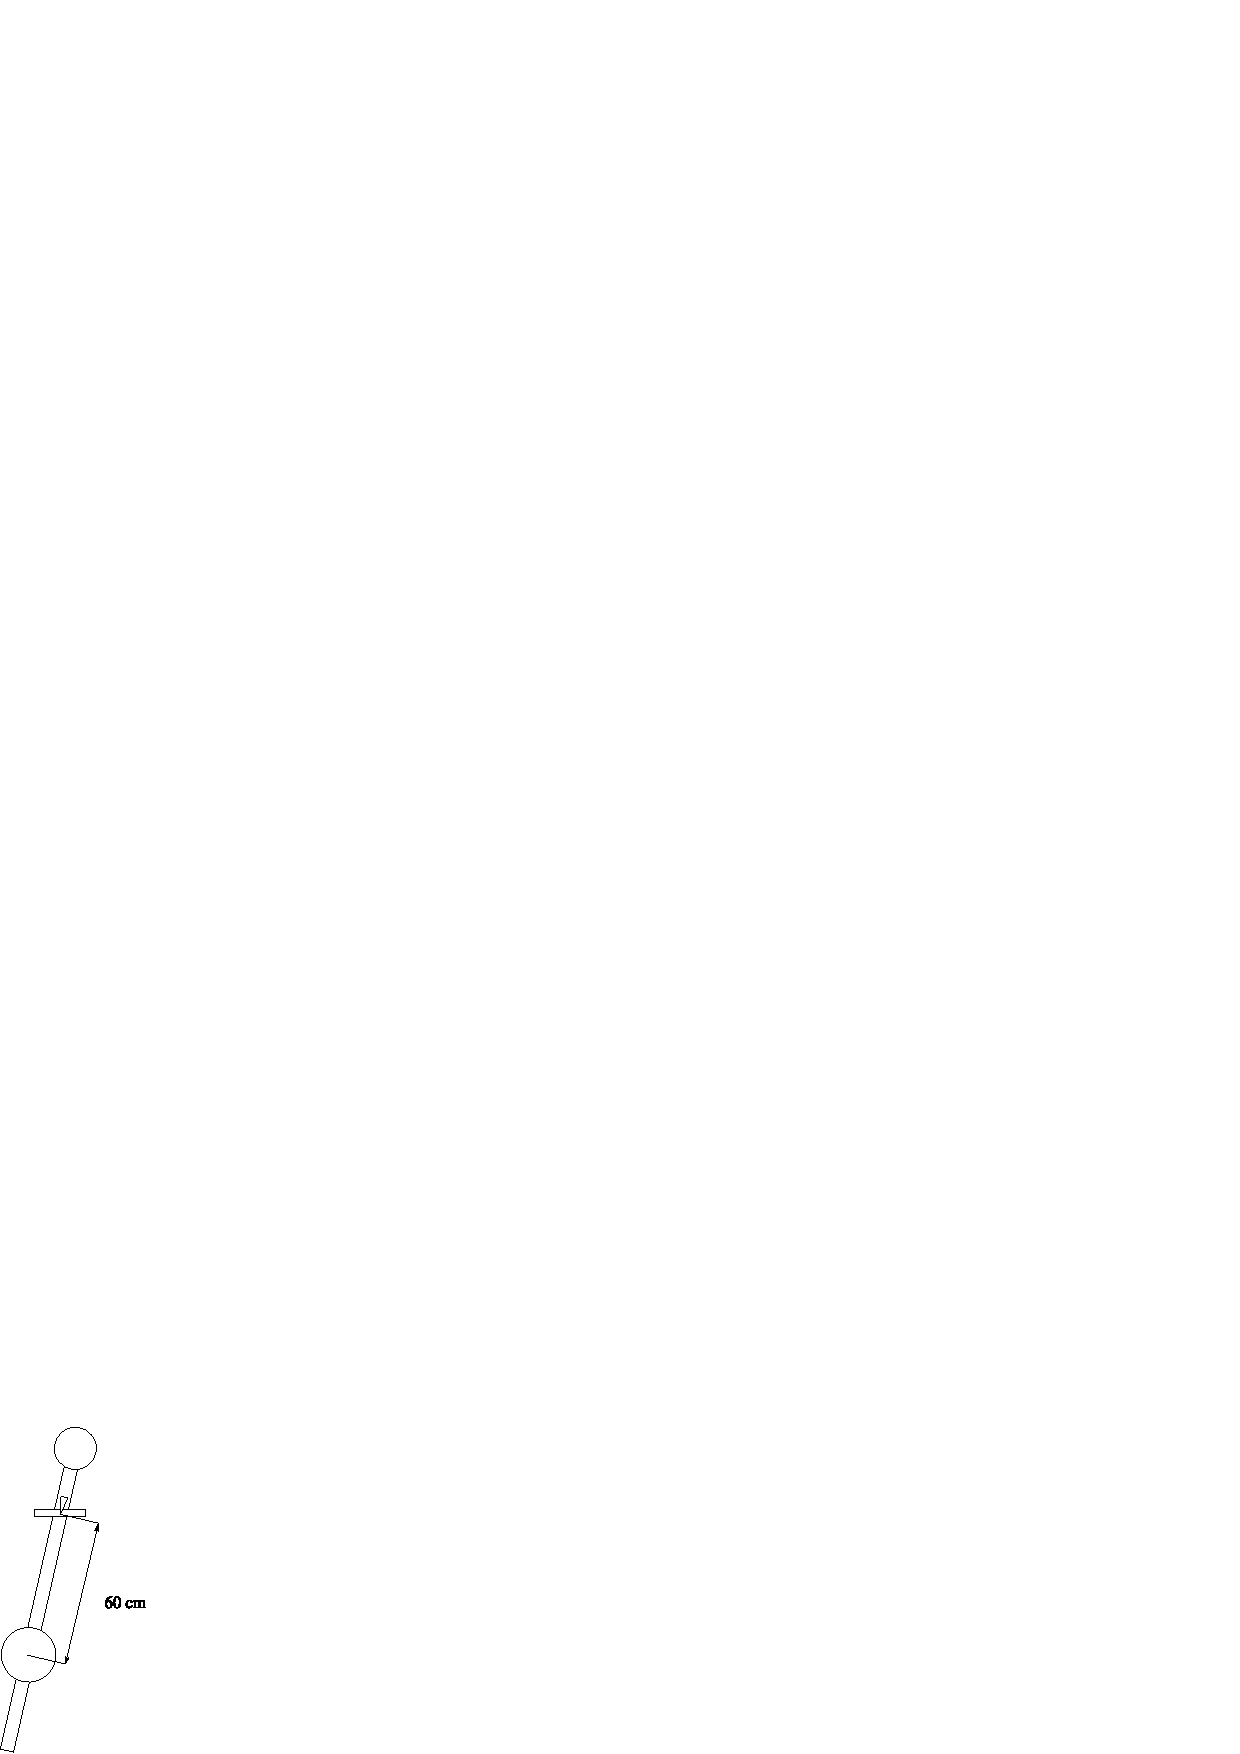
\includegraphics{disegno.jpg}
  \end{center}
  \caption{Rappresentazione schematica del pendolo.}\label{disegno}
\end{wrapfigure}
Lo strumento è un pendolo (vedi figura~\ref{disegno}), costituito da una barra di metallo a cui sono fissate due masse: una $60$~cm al di sotto del sostegno e un contrappeso al di sopra. Il pendolo oscilla su un coltello di acciaio temprato largo $5\cdot10^{-2}$~mm.

Nella prima parte dell'esperienza è stato utilizzato un cronometro manuale, con sensibilità di $10^{-3}$~s. Nella seconda parte, invece, il cronometro era dotato di un sistema di rilevazione automatico, ovvero una fotocellula sensibile al passaggio del pendolo nel punto più basso della traiettoria di oscillazione. Tale sistema ha una sensibiltà di $10^{-4}$~s ed è programmato in modo da registrare la durata di un periodo intero.
\section{Descrizione della metodologia di misura}
Sono stati registrati manualmente tre campioni di dati: un primo di 120 misure di una singola oscillazione completa (vedi tabella~\ref{tab100}), un secondo di 52 misure di due oscillazioni (vedi tabella~\subref{tab50}) e un terzo campione di 28 misure di quattro oscillazioni (vedi tabella~\subref{tab25}). Il tempo qui misurato come periodo è l'intervallo tra due arresti consecutivi del pendolo sullo stesso lato.

Con l'apparato automatico sono state raccolte prima 100, poi 999 misure. Il sistema rileva il tempo trascorso tra due passaggi consecutivi del pendolo nel punto più basso del suo movimento, ed è programmato per salvare dati relativi a un'oscillazione completa, e non ai semiperiodi.
\newpage
\section{Risultati sperimentali ed elaborazione dati}
I tempi registrati nei campioni sono riportati nelle tabelle successive. Per ogni campione è stato elaborato un istogramma suddividendo i dati in classi di frequenza dell'ampiezza di $15$~ms, messo a confronto con una distribuzione casuale gaussiana. Sono stati inoltre calcolati media aritmetica~$\bar{x}$, l'errore quadratico medio~$\sigma$ e l'errore della media~$\sigma_{\bar{x}}$. Nel campione relativo alle misure manuali della singola oscillazione, è stato individuato un valore esterno all'intervallo $[\bar{x} - 3\sigma,\bar{x} + 3\sigma]$ e quindi escluso.
\begin{table}[h!]\centering
\begin{tabular}{ c *3{r@{.}l}r@{ $\pm$ }l }
 \multicolumn{1}{ c }{n. misure $\times$ osc.}&
 \multicolumn{2}{c}{$\bar{x}$ (ms)}&
 \multicolumn{2}{c}{$\sigma$} &
 \multicolumn{2}{c}{$\sigma_{\bar{x}}$} &
 \multicolumn{2}{c}{risultato}\\
 \hline
 $120 \times 1$  	& 1936&47	&  63&64 	& 5&81 		&  1936.5  & 5.8\\
 $52 \times 2$  	& 3859&51 	&  88&07 	& 12&10 	&  3859.5  &12.1\\
 $28 \times 4$  	& 7711&79  	&   88&09  	&  16&65  	&   7711.8 &16.7\\
 $100$ (auto)		& 1927&21 	&  0&09 	& 0&01 		&  1927.21 &0.01\\
\end{tabular}
\end{table}\\
Ovvero, riportando i valori a un'oscillazione:
\begin{table}[h]\centering
\begin{tabular}{r r@{.}l @{ $\pm$ } r@{.}l @{ ms}}
120 & 1936&5 & 5&8 \\
52 & 1929&7 & 6&0  \\
28 & 1927&9 & 4&1  \\
100a & 1927&21 & 0&01  \\
\end{tabular}
\end{table}\\
\`{E} stata calcolata la compatibilità $\lambda$ di tali valori, secondo la formula:
\begin{equation*}
 \lambda_{i,j} = \dfrac{|\bar{x}_i - \bar{x}_j|}{\sqrt{\sigma_{\bar{x}_i}^2 + \sigma_{\bar{x}_j}^2}}
\end{equation*}
Con i seguenti risultati:
\begin{table}[h]\centering
\begin{tabular}{@{}r|r@{.}l r@{.}l r@{.}l}
 $\lambda$	&
 \multicolumn{2}{c}{120}
&   \multicolumn{2}{c}{52}
&   \multicolumn{2}{c}{28}  		\\
 \hline
 100a 		&  1&59 	&  0&42 	& 0&18 		\\
 28   		&  1&19 	&  0&25 	& \multicolumn{2}{c}{} \\
 52  	 	&  0&80 	& \multicolumn{2}{c}{}	& \multicolumn{2}{c}{}		 \\
\end{tabular}
\end{table}\\
La compatibilità si dice buona se ha valore compreso tra $0$ e $1$, mediocre tra~$1$~e~$2$~e scarsa tra~$2$~e~$3$.
I dati sono stati anche organizzati in istogrammi e confrontati con la curva gaussiana:
\begin{equation*}
 f(x) = \dfrac{N\Delta x}{\sigma \sqrt{2\pi}}\exp \left\{-\dfrac 1 2 \Big({\dfrac{x-\bar{x}}{\sigma}}\Big)^2\right\}
\end{equation*}
Dove $\Delta x$ è l'ampiezza delle classi di frequenza (15 ms), $N$ il numero totale di osservazioni e $\bar{x}$ la media aritmetica.
\section{Discussione dei risultati}
L'indice di compatibilità rispetto alle misure automatiche, gli errori sulle misure e sulla media mostrano chiaramente che la stima migliore è quella data dalle osservazioni su più periodi consecutivi. Ciò è giustificato dal fatto che l'errore $\sigma$ dovuto soprattutto al tempo di reazione dell'osservatore, è pressapoco costante su ogni misura, ma viene distribuito su un maggior numero di periodi, dunque influisce meno sulla stima della singola oscillazione. A conferma 

Per quanto riguarda i grafici, la distribuzione casuale degli errori è più evidente nelle misure di singole oscillazioni (come si vede dal grafico~\ref{gr1}) nonostante il picco sia spostato di circa 20~ms a destra. Il secondo grafico~(\ref{gr2}) rispetta meglio la stima centrale, anche se la scarsità di dati produce numerose irregolarità, che sono ancora più evidenti nel terzo istogramma~(\ref{gr4}) dove il picco di frequenza è quasi isolato. In tutti e tre i grafici si nota inoltre che la forma dell'istogramma presenta massimi secondari in eccesso di circa 50~ms.

Più interessante risulta il grafico delle 999 rilevazioni automatiche, in cui il massimo è nettamente spostato a sinistra e la distribuzione non è affatto simmetrica per la presenza di un errore sistematico dovuto all'approssimazione del periodo di oscillazione come indipendente dall'ampiezza dell'angolo. Una migliore approssimazione sarebbe infatti:
\begin{equation*}
 T = T_0\left(1+\dfrac{\alpha^2}{16}+\dfrac{9\alpha^4}{1024}+\cdots\right)
\end{equation*}
Come testimonia anche il grafico~\ref{gr1000} con le misure in ordine di rilevazione, il periodo diminuisce con lo smorzamento dell'oscillazione di circa 3~ms dopo 1000 periodi, ma non in modo lineare, ovvero in modo sempre meno marcato. Di conseguenza l'errore casuale è più evidente nelle ultime misure, che risultano più irregolari. Per lo stesso motivo l'istogramma delle frequenze si avvicina a una distribuzione casuale solo nella sua parte sinistra. Il grafico~\ref{sist} mostra una gaussiana con i dati di tutte le 999 misure, evidentemente inadeguata a rendere conto della distribuzione per la presenza dell'errore sistematico, mentre la gaussiana relativa ai dati delle ultime 500 osservazioni risulta meglio centrata sul massimo e più coerente con le misure intorno.

La serie di 999~misure automatiche è stato poi analizzato suddividendolo in dieci blocchi (vedi tabella~\ref{blocchi}), cosa che evidenzia ancora una volta la diminuzione della durata delle oscillazioni.

\section{Conclusioni}
L'esperienza dimostra chiaramente che per misurare manualmente il periodo di un pendolo è utile raggruppare più oscillazioni in una stessa misura, per distribuire l'effetto dell'imprecisione dovuta alla prontezza dell'operatore, che si può quantificare nell'ordine di grandezza di $10^{-1} s$. Una strumentazione elettronica permette invece di ridurre tali errori di tre ordini di grandezza rendendo possibile lo studio di errori sistematici dovuti allo smorzamento dell'ampiezza di oscillazione.
\newpage
\section{Appendice}
   \begin {figure}[hp]\caption{Campione di 120 misure di un'oscillazione.}\label{gr1}
      \begin{center}
        % GNUPLOT: LaTeX picture
\setlength{\unitlength}{0.240900pt}
\ifx\plotpoint\undefined\newsavebox{\plotpoint}\fi
\begin{picture}(1049,629)(0,0)
\sbox{\plotpoint}{\rule[-0.200pt]{0.400pt}{0.400pt}}%
\put(100,123){\makebox(0,0)[r]{ 0}}
\put(120.0,123.0){\rule[-0.200pt]{4.818pt}{0.400pt}}
\put(100,175){\makebox(0,0)[r]{ 2}}
\put(120.0,175.0){\rule[-0.200pt]{4.818pt}{0.400pt}}
\put(100,227){\makebox(0,0)[r]{ 4}}
\put(120.0,227.0){\rule[-0.200pt]{4.818pt}{0.400pt}}
\put(100,279){\makebox(0,0)[r]{ 6}}
\put(120.0,279.0){\rule[-0.200pt]{4.818pt}{0.400pt}}
\put(100,331){\makebox(0,0)[r]{ 8}}
\put(120.0,331.0){\rule[-0.200pt]{4.818pt}{0.400pt}}
\put(100,382){\makebox(0,0)[r]{ 10}}
\put(120.0,382.0){\rule[-0.200pt]{4.818pt}{0.400pt}}
\put(100,434){\makebox(0,0)[r]{ 12}}
\put(120.0,434.0){\rule[-0.200pt]{4.818pt}{0.400pt}}
\put(100,486){\makebox(0,0)[r]{ 14}}
\put(120.0,486.0){\rule[-0.200pt]{4.818pt}{0.400pt}}
\put(100,538){\makebox(0,0)[r]{ 16}}
\put(120.0,538.0){\rule[-0.200pt]{4.818pt}{0.400pt}}
\put(100,590){\makebox(0,0)[r]{ 18}}
\put(120.0,590.0){\rule[-0.200pt]{4.818pt}{0.400pt}}
\put(120,82){\makebox(0,0){ 1700}}
\put(120.0,123.0){\rule[-0.200pt]{0.400pt}{4.818pt}}
\put(164.0,123.0){\rule[-0.200pt]{0.400pt}{2.409pt}}
\put(209.0,123.0){\rule[-0.200pt]{0.400pt}{2.409pt}}
\put(253.0,123.0){\rule[-0.200pt]{0.400pt}{2.409pt}}
\put(298,82){\makebox(0,0){ 1800}}
\put(298.0,123.0){\rule[-0.200pt]{0.400pt}{4.818pt}}
\put(342.0,123.0){\rule[-0.200pt]{0.400pt}{2.409pt}}
\put(387.0,123.0){\rule[-0.200pt]{0.400pt}{2.409pt}}
\put(431.0,123.0){\rule[-0.200pt]{0.400pt}{2.409pt}}
\put(476,82){\makebox(0,0){ 1900}}
\put(476.0,123.0){\rule[-0.200pt]{0.400pt}{4.818pt}}
\put(520.0,123.0){\rule[-0.200pt]{0.400pt}{2.409pt}}
\put(565.0,123.0){\rule[-0.200pt]{0.400pt}{2.409pt}}
\put(609.0,123.0){\rule[-0.200pt]{0.400pt}{2.409pt}}
\put(653,82){\makebox(0,0){ 2000}}
\put(653.0,123.0){\rule[-0.200pt]{0.400pt}{4.818pt}}
\put(698.0,123.0){\rule[-0.200pt]{0.400pt}{2.409pt}}
\put(742.0,123.0){\rule[-0.200pt]{0.400pt}{2.409pt}}
\put(787.0,123.0){\rule[-0.200pt]{0.400pt}{2.409pt}}
\put(831,82){\makebox(0,0){ 2100}}
\put(831.0,123.0){\rule[-0.200pt]{0.400pt}{4.818pt}}
\put(876.0,123.0){\rule[-0.200pt]{0.400pt}{2.409pt}}
\put(920.0,123.0){\rule[-0.200pt]{0.400pt}{2.409pt}}
\put(965.0,123.0){\rule[-0.200pt]{0.400pt}{2.409pt}}
\put(1009,82){\makebox(0,0){ 2200}}
\put(1009.0,123.0){\rule[-0.200pt]{0.400pt}{4.818pt}}
\put(120.0,123.0){\rule[-0.200pt]{0.400pt}{112.500pt}}
\put(120.0,123.0){\rule[-0.200pt]{214.160pt}{0.400pt}}
\put(1009.0,123.0){\rule[-0.200pt]{0.400pt}{112.500pt}}
\put(120.0,590.0){\rule[-0.200pt]{214.160pt}{0.400pt}}
\put(564,21){\makebox(0,0){ms}}
\put(120,123){\usebox{\plotpoint}}
\put(147,122.67){\rule{2.168pt}{0.400pt}}
\multiput(147.00,122.17)(4.500,1.000){2}{\rule{1.084pt}{0.400pt}}
\put(120.0,123.0){\rule[-0.200pt]{6.504pt}{0.400pt}}
\put(183,123.67){\rule{2.168pt}{0.400pt}}
\multiput(183.00,123.17)(4.500,1.000){2}{\rule{1.084pt}{0.400pt}}
\put(156.0,124.0){\rule[-0.200pt]{6.504pt}{0.400pt}}
\put(201,124.67){\rule{2.168pt}{0.400pt}}
\multiput(201.00,124.17)(4.500,1.000){2}{\rule{1.084pt}{0.400pt}}
\put(210,125.67){\rule{2.168pt}{0.400pt}}
\multiput(210.00,125.17)(4.500,1.000){2}{\rule{1.084pt}{0.400pt}}
\put(219,126.67){\rule{2.168pt}{0.400pt}}
\multiput(219.00,126.17)(4.500,1.000){2}{\rule{1.084pt}{0.400pt}}
\put(228,127.67){\rule{2.168pt}{0.400pt}}
\multiput(228.00,127.17)(4.500,1.000){2}{\rule{1.084pt}{0.400pt}}
\put(237,128.67){\rule{2.168pt}{0.400pt}}
\multiput(237.00,128.17)(4.500,1.000){2}{\rule{1.084pt}{0.400pt}}
\put(246,130.17){\rule{1.900pt}{0.400pt}}
\multiput(246.00,129.17)(5.056,2.000){2}{\rule{0.950pt}{0.400pt}}
\put(255,132.17){\rule{1.900pt}{0.400pt}}
\multiput(255.00,131.17)(5.056,2.000){2}{\rule{0.950pt}{0.400pt}}
\put(264,134.17){\rule{1.900pt}{0.400pt}}
\multiput(264.00,133.17)(5.056,2.000){2}{\rule{0.950pt}{0.400pt}}
\multiput(273.00,136.61)(1.802,0.447){3}{\rule{1.300pt}{0.108pt}}
\multiput(273.00,135.17)(6.302,3.000){2}{\rule{0.650pt}{0.400pt}}
\multiput(282.00,139.60)(1.212,0.468){5}{\rule{1.000pt}{0.113pt}}
\multiput(282.00,138.17)(6.924,4.000){2}{\rule{0.500pt}{0.400pt}}
\multiput(291.00,143.61)(1.802,0.447){3}{\rule{1.300pt}{0.108pt}}
\multiput(291.00,142.17)(6.302,3.000){2}{\rule{0.650pt}{0.400pt}}
\multiput(300.00,146.59)(0.933,0.477){7}{\rule{0.820pt}{0.115pt}}
\multiput(300.00,145.17)(7.298,5.000){2}{\rule{0.410pt}{0.400pt}}
\multiput(309.00,151.59)(0.933,0.477){7}{\rule{0.820pt}{0.115pt}}
\multiput(309.00,150.17)(7.298,5.000){2}{\rule{0.410pt}{0.400pt}}
\multiput(318.00,156.59)(0.762,0.482){9}{\rule{0.700pt}{0.116pt}}
\multiput(318.00,155.17)(7.547,6.000){2}{\rule{0.350pt}{0.400pt}}
\multiput(327.00,162.59)(0.762,0.482){9}{\rule{0.700pt}{0.116pt}}
\multiput(327.00,161.17)(7.547,6.000){2}{\rule{0.350pt}{0.400pt}}
\multiput(336.00,168.59)(0.569,0.485){11}{\rule{0.557pt}{0.117pt}}
\multiput(336.00,167.17)(6.844,7.000){2}{\rule{0.279pt}{0.400pt}}
\multiput(344.00,175.59)(0.560,0.488){13}{\rule{0.550pt}{0.117pt}}
\multiput(344.00,174.17)(7.858,8.000){2}{\rule{0.275pt}{0.400pt}}
\multiput(353.00,183.59)(0.495,0.489){15}{\rule{0.500pt}{0.118pt}}
\multiput(353.00,182.17)(7.962,9.000){2}{\rule{0.250pt}{0.400pt}}
\multiput(362.00,192.59)(0.495,0.489){15}{\rule{0.500pt}{0.118pt}}
\multiput(362.00,191.17)(7.962,9.000){2}{\rule{0.250pt}{0.400pt}}
\multiput(371.59,201.00)(0.489,0.553){15}{\rule{0.118pt}{0.544pt}}
\multiput(370.17,201.00)(9.000,8.870){2}{\rule{0.400pt}{0.272pt}}
\multiput(380.59,211.00)(0.489,0.611){15}{\rule{0.118pt}{0.589pt}}
\multiput(379.17,211.00)(9.000,9.778){2}{\rule{0.400pt}{0.294pt}}
\multiput(389.59,222.00)(0.489,0.611){15}{\rule{0.118pt}{0.589pt}}
\multiput(388.17,222.00)(9.000,9.778){2}{\rule{0.400pt}{0.294pt}}
\multiput(398.59,233.00)(0.489,0.611){15}{\rule{0.118pt}{0.589pt}}
\multiput(397.17,233.00)(9.000,9.778){2}{\rule{0.400pt}{0.294pt}}
\multiput(407.59,244.00)(0.489,0.669){15}{\rule{0.118pt}{0.633pt}}
\multiput(406.17,244.00)(9.000,10.685){2}{\rule{0.400pt}{0.317pt}}
\multiput(416.59,256.00)(0.489,0.669){15}{\rule{0.118pt}{0.633pt}}
\multiput(415.17,256.00)(9.000,10.685){2}{\rule{0.400pt}{0.317pt}}
\multiput(425.59,268.00)(0.489,0.728){15}{\rule{0.118pt}{0.678pt}}
\multiput(424.17,268.00)(9.000,11.593){2}{\rule{0.400pt}{0.339pt}}
\multiput(434.59,281.00)(0.489,0.669){15}{\rule{0.118pt}{0.633pt}}
\multiput(433.17,281.00)(9.000,10.685){2}{\rule{0.400pt}{0.317pt}}
\multiput(443.59,293.00)(0.489,0.611){15}{\rule{0.118pt}{0.589pt}}
\multiput(442.17,293.00)(9.000,9.778){2}{\rule{0.400pt}{0.294pt}}
\multiput(452.59,304.00)(0.489,0.669){15}{\rule{0.118pt}{0.633pt}}
\multiput(451.17,304.00)(9.000,10.685){2}{\rule{0.400pt}{0.317pt}}
\multiput(461.59,316.00)(0.489,0.553){15}{\rule{0.118pt}{0.544pt}}
\multiput(460.17,316.00)(9.000,8.870){2}{\rule{0.400pt}{0.272pt}}
\multiput(470.59,326.00)(0.489,0.553){15}{\rule{0.118pt}{0.544pt}}
\multiput(469.17,326.00)(9.000,8.870){2}{\rule{0.400pt}{0.272pt}}
\multiput(479.00,336.59)(0.495,0.489){15}{\rule{0.500pt}{0.118pt}}
\multiput(479.00,335.17)(7.962,9.000){2}{\rule{0.250pt}{0.400pt}}
\multiput(488.00,345.59)(0.560,0.488){13}{\rule{0.550pt}{0.117pt}}
\multiput(488.00,344.17)(7.858,8.000){2}{\rule{0.275pt}{0.400pt}}
\multiput(497.00,353.59)(0.762,0.482){9}{\rule{0.700pt}{0.116pt}}
\multiput(497.00,352.17)(7.547,6.000){2}{\rule{0.350pt}{0.400pt}}
\multiput(506.00,359.59)(0.933,0.477){7}{\rule{0.820pt}{0.115pt}}
\multiput(506.00,358.17)(7.298,5.000){2}{\rule{0.410pt}{0.400pt}}
\multiput(515.00,364.60)(1.212,0.468){5}{\rule{1.000pt}{0.113pt}}
\multiput(515.00,363.17)(6.924,4.000){2}{\rule{0.500pt}{0.400pt}}
\put(524,368.17){\rule{1.900pt}{0.400pt}}
\multiput(524.00,367.17)(5.056,2.000){2}{\rule{0.950pt}{0.400pt}}
\put(192.0,125.0){\rule[-0.200pt]{2.168pt}{0.400pt}}
\put(542,368.17){\rule{1.900pt}{0.400pt}}
\multiput(542.00,369.17)(5.056,-2.000){2}{\rule{0.950pt}{0.400pt}}
\multiput(551.00,366.95)(1.802,-0.447){3}{\rule{1.300pt}{0.108pt}}
\multiput(551.00,367.17)(6.302,-3.000){2}{\rule{0.650pt}{0.400pt}}
\multiput(560.00,363.94)(1.212,-0.468){5}{\rule{1.000pt}{0.113pt}}
\multiput(560.00,364.17)(6.924,-4.000){2}{\rule{0.500pt}{0.400pt}}
\multiput(569.00,359.93)(0.762,-0.482){9}{\rule{0.700pt}{0.116pt}}
\multiput(569.00,360.17)(7.547,-6.000){2}{\rule{0.350pt}{0.400pt}}
\multiput(578.00,353.93)(0.645,-0.485){11}{\rule{0.614pt}{0.117pt}}
\multiput(578.00,354.17)(7.725,-7.000){2}{\rule{0.307pt}{0.400pt}}
\multiput(587.00,346.93)(0.495,-0.489){15}{\rule{0.500pt}{0.118pt}}
\multiput(587.00,347.17)(7.962,-9.000){2}{\rule{0.250pt}{0.400pt}}
\multiput(596.59,336.74)(0.489,-0.553){15}{\rule{0.118pt}{0.544pt}}
\multiput(595.17,337.87)(9.000,-8.870){2}{\rule{0.400pt}{0.272pt}}
\multiput(605.59,326.74)(0.489,-0.553){15}{\rule{0.118pt}{0.544pt}}
\multiput(604.17,327.87)(9.000,-8.870){2}{\rule{0.400pt}{0.272pt}}
\multiput(614.59,316.56)(0.489,-0.611){15}{\rule{0.118pt}{0.589pt}}
\multiput(613.17,317.78)(9.000,-9.778){2}{\rule{0.400pt}{0.294pt}}
\multiput(623.59,305.37)(0.489,-0.669){15}{\rule{0.118pt}{0.633pt}}
\multiput(622.17,306.69)(9.000,-10.685){2}{\rule{0.400pt}{0.317pt}}
\multiput(632.59,293.37)(0.489,-0.669){15}{\rule{0.118pt}{0.633pt}}
\multiput(631.17,294.69)(9.000,-10.685){2}{\rule{0.400pt}{0.317pt}}
\multiput(641.59,281.37)(0.489,-0.669){15}{\rule{0.118pt}{0.633pt}}
\multiput(640.17,282.69)(9.000,-10.685){2}{\rule{0.400pt}{0.317pt}}
\multiput(650.59,269.37)(0.489,-0.669){15}{\rule{0.118pt}{0.633pt}}
\multiput(649.17,270.69)(9.000,-10.685){2}{\rule{0.400pt}{0.317pt}}
\multiput(659.59,257.37)(0.489,-0.669){15}{\rule{0.118pt}{0.633pt}}
\multiput(658.17,258.69)(9.000,-10.685){2}{\rule{0.400pt}{0.317pt}}
\multiput(668.59,245.37)(0.489,-0.669){15}{\rule{0.118pt}{0.633pt}}
\multiput(667.17,246.69)(9.000,-10.685){2}{\rule{0.400pt}{0.317pt}}
\multiput(677.59,233.56)(0.489,-0.611){15}{\rule{0.118pt}{0.589pt}}
\multiput(676.17,234.78)(9.000,-9.778){2}{\rule{0.400pt}{0.294pt}}
\multiput(686.59,222.56)(0.489,-0.611){15}{\rule{0.118pt}{0.589pt}}
\multiput(685.17,223.78)(9.000,-9.778){2}{\rule{0.400pt}{0.294pt}}
\multiput(695.59,211.74)(0.489,-0.553){15}{\rule{0.118pt}{0.544pt}}
\multiput(694.17,212.87)(9.000,-8.870){2}{\rule{0.400pt}{0.272pt}}
\multiput(704.59,201.74)(0.489,-0.553){15}{\rule{0.118pt}{0.544pt}}
\multiput(703.17,202.87)(9.000,-8.870){2}{\rule{0.400pt}{0.272pt}}
\multiput(713.00,192.93)(0.495,-0.489){15}{\rule{0.500pt}{0.118pt}}
\multiput(713.00,193.17)(7.962,-9.000){2}{\rule{0.250pt}{0.400pt}}
\multiput(722.00,183.93)(0.560,-0.488){13}{\rule{0.550pt}{0.117pt}}
\multiput(722.00,184.17)(7.858,-8.000){2}{\rule{0.275pt}{0.400pt}}
\multiput(731.00,175.93)(0.645,-0.485){11}{\rule{0.614pt}{0.117pt}}
\multiput(731.00,176.17)(7.725,-7.000){2}{\rule{0.307pt}{0.400pt}}
\multiput(740.00,168.93)(0.645,-0.485){11}{\rule{0.614pt}{0.117pt}}
\multiput(740.00,169.17)(7.725,-7.000){2}{\rule{0.307pt}{0.400pt}}
\multiput(749.00,161.93)(0.762,-0.482){9}{\rule{0.700pt}{0.116pt}}
\multiput(749.00,162.17)(7.547,-6.000){2}{\rule{0.350pt}{0.400pt}}
\multiput(758.00,155.93)(0.933,-0.477){7}{\rule{0.820pt}{0.115pt}}
\multiput(758.00,156.17)(7.298,-5.000){2}{\rule{0.410pt}{0.400pt}}
\multiput(767.00,150.94)(1.212,-0.468){5}{\rule{1.000pt}{0.113pt}}
\multiput(767.00,151.17)(6.924,-4.000){2}{\rule{0.500pt}{0.400pt}}
\multiput(776.00,146.94)(1.212,-0.468){5}{\rule{1.000pt}{0.113pt}}
\multiput(776.00,147.17)(6.924,-4.000){2}{\rule{0.500pt}{0.400pt}}
\multiput(785.00,142.94)(1.066,-0.468){5}{\rule{0.900pt}{0.113pt}}
\multiput(785.00,143.17)(6.132,-4.000){2}{\rule{0.450pt}{0.400pt}}
\multiput(793.00,138.95)(1.802,-0.447){3}{\rule{1.300pt}{0.108pt}}
\multiput(793.00,139.17)(6.302,-3.000){2}{\rule{0.650pt}{0.400pt}}
\put(802,135.17){\rule{1.900pt}{0.400pt}}
\multiput(802.00,136.17)(5.056,-2.000){2}{\rule{0.950pt}{0.400pt}}
\multiput(811.00,133.95)(1.802,-0.447){3}{\rule{1.300pt}{0.108pt}}
\multiput(811.00,134.17)(6.302,-3.000){2}{\rule{0.650pt}{0.400pt}}
\put(820,130.67){\rule{2.168pt}{0.400pt}}
\multiput(820.00,131.17)(4.500,-1.000){2}{\rule{1.084pt}{0.400pt}}
\put(829,129.17){\rule{1.900pt}{0.400pt}}
\multiput(829.00,130.17)(5.056,-2.000){2}{\rule{0.950pt}{0.400pt}}
\put(838,127.67){\rule{2.168pt}{0.400pt}}
\multiput(838.00,128.17)(4.500,-1.000){2}{\rule{1.084pt}{0.400pt}}
\put(847,126.67){\rule{2.168pt}{0.400pt}}
\multiput(847.00,127.17)(4.500,-1.000){2}{\rule{1.084pt}{0.400pt}}
\put(856,125.67){\rule{2.168pt}{0.400pt}}
\multiput(856.00,126.17)(4.500,-1.000){2}{\rule{1.084pt}{0.400pt}}
\put(865,124.67){\rule{2.168pt}{0.400pt}}
\multiput(865.00,125.17)(4.500,-1.000){2}{\rule{1.084pt}{0.400pt}}
\put(533.0,370.0){\rule[-0.200pt]{2.168pt}{0.400pt}}
\put(883,123.67){\rule{2.168pt}{0.400pt}}
\multiput(883.00,124.17)(4.500,-1.000){2}{\rule{1.084pt}{0.400pt}}
\put(874.0,125.0){\rule[-0.200pt]{2.168pt}{0.400pt}}
\put(919,122.67){\rule{2.168pt}{0.400pt}}
\multiput(919.00,123.17)(4.500,-1.000){2}{\rule{1.084pt}{0.400pt}}
\put(892.0,124.0){\rule[-0.200pt]{6.504pt}{0.400pt}}
\put(928.0,123.0){\rule[-0.200pt]{19.513pt}{0.400pt}}
\sbox{\plotpoint}{\rule[-0.400pt]{0.800pt}{0.800pt}}%
\put(254,175){\usebox{\plotpoint}}
\put(254.0,175.0){\rule[-0.400pt]{5.782pt}{0.800pt}}
\put(278.0,123.0){\rule[-0.400pt]{0.800pt}{12.527pt}}
\put(278.0,123.0){\rule[-0.400pt]{5.541pt}{0.800pt}}
\put(301.0,123.0){\rule[-0.400pt]{0.800pt}{6.263pt}}
\put(301.0,149.0){\rule[-0.400pt]{16.622pt}{0.800pt}}
\put(370.0,149.0){\rule[-0.400pt]{0.800pt}{31.317pt}}
\put(370.0,279.0){\rule[-0.400pt]{5.541pt}{0.800pt}}
\put(393.0,279.0){\rule[-0.400pt]{0.800pt}{12.527pt}}
\put(393.0,331.0){\rule[-0.400pt]{5.541pt}{0.800pt}}
\put(416.0,253.0){\rule[-0.400pt]{0.800pt}{18.790pt}}
\put(416.0,253.0){\rule[-0.400pt]{11.081pt}{0.800pt}}
\put(462.0,253.0){\rule[-0.400pt]{0.800pt}{12.527pt}}
\put(462.0,305.0){\rule[-0.400pt]{5.782pt}{0.800pt}}
\put(486.0,305.0){\rule[-0.400pt]{0.800pt}{12.286pt}}
\put(486.0,356.0){\rule[-0.400pt]{5.541pt}{0.800pt}}
\put(509.0,279.0){\rule[-0.400pt]{0.800pt}{18.549pt}}
\put(509.0,279.0){\rule[-0.400pt]{5.541pt}{0.800pt}}
\put(532.0,279.0){\rule[-0.400pt]{0.800pt}{31.076pt}}
\put(532.0,408.0){\rule[-0.400pt]{5.541pt}{0.800pt}}
\put(555.0,356.0){\rule[-0.400pt]{0.800pt}{12.527pt}}
\put(555.0,356.0){\rule[-0.400pt]{5.541pt}{0.800pt}}
\put(578.0,356.0){\rule[-0.400pt]{0.800pt}{31.317pt}}
\put(578.0,486.0){\rule[-0.400pt]{5.541pt}{0.800pt}}
\put(601.0,356.0){\rule[-0.400pt]{0.800pt}{31.317pt}}
\put(601.0,356.0){\rule[-0.400pt]{5.541pt}{0.800pt}}
\put(624.0,227.0){\rule[-0.400pt]{0.800pt}{31.076pt}}
\put(624.0,227.0){\rule[-0.400pt]{11.322pt}{0.800pt}}
\put(671.0,227.0){\rule[-0.400pt]{0.800pt}{18.790pt}}
\put(671.0,305.0){\rule[-0.400pt]{5.541pt}{0.800pt}}
\put(694.0,201.0){\rule[-0.400pt]{0.800pt}{25.054pt}}
\put(694.0,201.0){\rule[-0.400pt]{5.541pt}{0.800pt}}
\put(717.0,175.0){\rule[-0.400pt]{0.800pt}{6.263pt}}
\put(717.0,175.0){\rule[-0.400pt]{16.622pt}{0.800pt}}
\put(786.0,149.0){\rule[-0.400pt]{0.800pt}{6.263pt}}
\put(786.0,149.0){\rule[-0.400pt]{5.541pt}{0.800pt}}
\put(809.0,123.0){\rule[-0.400pt]{0.800pt}{6.263pt}}
\put(809.0,123.0){\rule[-0.400pt]{16.863pt}{0.800pt}}
\put(879.0,123.0){\rule[-0.400pt]{0.800pt}{6.263pt}}
\put(879.0,149.0){\rule[-0.400pt]{5.541pt}{0.800pt}}
\put(902.0,123.0){\rule[-0.400pt]{0.800pt}{6.263pt}}
\put(902.0,123.0){\rule[-0.400pt]{5.541pt}{0.800pt}}
\sbox{\plotpoint}{\rule[-0.200pt]{0.400pt}{0.400pt}}%
\put(120.0,123.0){\rule[-0.200pt]{0.400pt}{112.500pt}}
\put(120.0,123.0){\rule[-0.200pt]{214.160pt}{0.400pt}}
\put(1009.0,123.0){\rule[-0.200pt]{0.400pt}{112.500pt}}
\put(120.0,590.0){\rule[-0.200pt]{214.160pt}{0.400pt}}
\end{picture}

      \end{center}
    \end {figure}
      \begin {figure}[hp]\caption{Campione di 52 misure di due oscillazioni.}\label{gr2}
      \begin{center}
        % GNUPLOT: LaTeX picture
\setlength{\unitlength}{0.240900pt}
\ifx\plotpoint\undefined\newsavebox{\plotpoint}\fi
\begin{picture}(1049,629)(0,0)
\sbox{\plotpoint}{\rule[-0.200pt]{0.400pt}{0.400pt}}%
\put(80,123){\makebox(0,0)[r]{ 0}}
\put(100.0,123.0){\rule[-0.200pt]{4.818pt}{0.400pt}}
\put(80,190){\makebox(0,0)[r]{ 1}}
\put(100.0,190.0){\rule[-0.200pt]{4.818pt}{0.400pt}}
\put(80,256){\makebox(0,0)[r]{ 2}}
\put(100.0,256.0){\rule[-0.200pt]{4.818pt}{0.400pt}}
\put(80,323){\makebox(0,0)[r]{ 3}}
\put(100.0,323.0){\rule[-0.200pt]{4.818pt}{0.400pt}}
\put(80,390){\makebox(0,0)[r]{ 4}}
\put(100.0,390.0){\rule[-0.200pt]{4.818pt}{0.400pt}}
\put(80,457){\makebox(0,0)[r]{ 5}}
\put(100.0,457.0){\rule[-0.200pt]{4.818pt}{0.400pt}}
\put(80,523){\makebox(0,0)[r]{ 6}}
\put(100.0,523.0){\rule[-0.200pt]{4.818pt}{0.400pt}}
\put(80,590){\makebox(0,0)[r]{ 7}}
\put(100.0,590.0){\rule[-0.200pt]{4.818pt}{0.400pt}}
\put(100,82){\makebox(0,0){ 3600}}
\put(100.0,123.0){\rule[-0.200pt]{0.400pt}{4.818pt}}
\put(145.0,123.0){\rule[-0.200pt]{0.400pt}{2.409pt}}
\put(191.0,123.0){\rule[-0.200pt]{0.400pt}{2.409pt}}
\put(236.0,123.0){\rule[-0.200pt]{0.400pt}{2.409pt}}
\put(282,82){\makebox(0,0){ 3700}}
\put(282.0,123.0){\rule[-0.200pt]{0.400pt}{4.818pt}}
\put(327.0,123.0){\rule[-0.200pt]{0.400pt}{2.409pt}}
\put(373.0,123.0){\rule[-0.200pt]{0.400pt}{2.409pt}}
\put(418.0,123.0){\rule[-0.200pt]{0.400pt}{2.409pt}}
\put(464,82){\makebox(0,0){ 3800}}
\put(464.0,123.0){\rule[-0.200pt]{0.400pt}{4.818pt}}
\put(509.0,123.0){\rule[-0.200pt]{0.400pt}{2.409pt}}
\put(555.0,123.0){\rule[-0.200pt]{0.400pt}{2.409pt}}
\put(600.0,123.0){\rule[-0.200pt]{0.400pt}{2.409pt}}
\put(645,82){\makebox(0,0){ 3900}}
\put(645.0,123.0){\rule[-0.200pt]{0.400pt}{4.818pt}}
\put(691.0,123.0){\rule[-0.200pt]{0.400pt}{2.409pt}}
\put(736.0,123.0){\rule[-0.200pt]{0.400pt}{2.409pt}}
\put(782.0,123.0){\rule[-0.200pt]{0.400pt}{2.409pt}}
\put(827,82){\makebox(0,0){ 4000}}
\put(827.0,123.0){\rule[-0.200pt]{0.400pt}{4.818pt}}
\put(873.0,123.0){\rule[-0.200pt]{0.400pt}{2.409pt}}
\put(918.0,123.0){\rule[-0.200pt]{0.400pt}{2.409pt}}
\put(964.0,123.0){\rule[-0.200pt]{0.400pt}{2.409pt}}
\put(1009,82){\makebox(0,0){ 4100}}
\put(1009.0,123.0){\rule[-0.200pt]{0.400pt}{4.818pt}}
\put(100.0,123.0){\rule[-0.200pt]{0.400pt}{112.500pt}}
\put(100.0,123.0){\rule[-0.200pt]{218.978pt}{0.400pt}}
\put(1009.0,123.0){\rule[-0.200pt]{0.400pt}{112.500pt}}
\put(100.0,590.0){\rule[-0.200pt]{218.978pt}{0.400pt}}
\put(554,21){\makebox(0,0){ms}}
\put(100,126){\usebox{\plotpoint}}
\put(100,125.67){\rule{2.168pt}{0.400pt}}
\multiput(100.00,125.17)(4.500,1.000){2}{\rule{1.084pt}{0.400pt}}
\put(118,126.67){\rule{2.409pt}{0.400pt}}
\multiput(118.00,126.17)(5.000,1.000){2}{\rule{1.204pt}{0.400pt}}
\put(128,127.67){\rule{2.168pt}{0.400pt}}
\multiput(128.00,127.17)(4.500,1.000){2}{\rule{1.084pt}{0.400pt}}
\put(137,128.67){\rule{2.168pt}{0.400pt}}
\multiput(137.00,128.17)(4.500,1.000){2}{\rule{1.084pt}{0.400pt}}
\put(146,129.67){\rule{2.168pt}{0.400pt}}
\multiput(146.00,129.17)(4.500,1.000){2}{\rule{1.084pt}{0.400pt}}
\put(155,130.67){\rule{2.168pt}{0.400pt}}
\multiput(155.00,130.17)(4.500,1.000){2}{\rule{1.084pt}{0.400pt}}
\put(164,132.17){\rule{1.900pt}{0.400pt}}
\multiput(164.00,131.17)(5.056,2.000){2}{\rule{0.950pt}{0.400pt}}
\put(173,134.17){\rule{2.100pt}{0.400pt}}
\multiput(173.00,133.17)(5.641,2.000){2}{\rule{1.050pt}{0.400pt}}
\put(183,135.67){\rule{2.168pt}{0.400pt}}
\multiput(183.00,135.17)(4.500,1.000){2}{\rule{1.084pt}{0.400pt}}
\put(192,137.17){\rule{1.900pt}{0.400pt}}
\multiput(192.00,136.17)(5.056,2.000){2}{\rule{0.950pt}{0.400pt}}
\multiput(201.00,139.61)(1.802,0.447){3}{\rule{1.300pt}{0.108pt}}
\multiput(201.00,138.17)(6.302,3.000){2}{\rule{0.650pt}{0.400pt}}
\put(210,142.17){\rule{1.900pt}{0.400pt}}
\multiput(210.00,141.17)(5.056,2.000){2}{\rule{0.950pt}{0.400pt}}
\multiput(219.00,144.61)(2.025,0.447){3}{\rule{1.433pt}{0.108pt}}
\multiput(219.00,143.17)(7.025,3.000){2}{\rule{0.717pt}{0.400pt}}
\multiput(229.00,147.61)(1.802,0.447){3}{\rule{1.300pt}{0.108pt}}
\multiput(229.00,146.17)(6.302,3.000){2}{\rule{0.650pt}{0.400pt}}
\multiput(238.00,150.60)(1.212,0.468){5}{\rule{1.000pt}{0.113pt}}
\multiput(238.00,149.17)(6.924,4.000){2}{\rule{0.500pt}{0.400pt}}
\multiput(247.00,154.61)(1.802,0.447){3}{\rule{1.300pt}{0.108pt}}
\multiput(247.00,153.17)(6.302,3.000){2}{\rule{0.650pt}{0.400pt}}
\multiput(256.00,157.60)(1.212,0.468){5}{\rule{1.000pt}{0.113pt}}
\multiput(256.00,156.17)(6.924,4.000){2}{\rule{0.500pt}{0.400pt}}
\multiput(265.00,161.59)(0.933,0.477){7}{\rule{0.820pt}{0.115pt}}
\multiput(265.00,160.17)(7.298,5.000){2}{\rule{0.410pt}{0.400pt}}
\multiput(274.00,166.59)(1.044,0.477){7}{\rule{0.900pt}{0.115pt}}
\multiput(274.00,165.17)(8.132,5.000){2}{\rule{0.450pt}{0.400pt}}
\multiput(284.00,171.59)(0.933,0.477){7}{\rule{0.820pt}{0.115pt}}
\multiput(284.00,170.17)(7.298,5.000){2}{\rule{0.410pt}{0.400pt}}
\multiput(293.00,176.59)(0.933,0.477){7}{\rule{0.820pt}{0.115pt}}
\multiput(293.00,175.17)(7.298,5.000){2}{\rule{0.410pt}{0.400pt}}
\multiput(302.00,181.59)(0.762,0.482){9}{\rule{0.700pt}{0.116pt}}
\multiput(302.00,180.17)(7.547,6.000){2}{\rule{0.350pt}{0.400pt}}
\multiput(311.00,187.59)(0.762,0.482){9}{\rule{0.700pt}{0.116pt}}
\multiput(311.00,186.17)(7.547,6.000){2}{\rule{0.350pt}{0.400pt}}
\multiput(320.00,193.59)(0.852,0.482){9}{\rule{0.767pt}{0.116pt}}
\multiput(320.00,192.17)(8.409,6.000){2}{\rule{0.383pt}{0.400pt}}
\multiput(330.00,199.59)(0.645,0.485){11}{\rule{0.614pt}{0.117pt}}
\multiput(330.00,198.17)(7.725,7.000){2}{\rule{0.307pt}{0.400pt}}
\multiput(339.00,206.59)(0.645,0.485){11}{\rule{0.614pt}{0.117pt}}
\multiput(339.00,205.17)(7.725,7.000){2}{\rule{0.307pt}{0.400pt}}
\multiput(348.00,213.59)(0.560,0.488){13}{\rule{0.550pt}{0.117pt}}
\multiput(348.00,212.17)(7.858,8.000){2}{\rule{0.275pt}{0.400pt}}
\multiput(357.00,221.59)(0.645,0.485){11}{\rule{0.614pt}{0.117pt}}
\multiput(357.00,220.17)(7.725,7.000){2}{\rule{0.307pt}{0.400pt}}
\multiput(366.00,228.59)(0.560,0.488){13}{\rule{0.550pt}{0.117pt}}
\multiput(366.00,227.17)(7.858,8.000){2}{\rule{0.275pt}{0.400pt}}
\multiput(375.00,236.59)(0.626,0.488){13}{\rule{0.600pt}{0.117pt}}
\multiput(375.00,235.17)(8.755,8.000){2}{\rule{0.300pt}{0.400pt}}
\multiput(385.00,244.59)(0.495,0.489){15}{\rule{0.500pt}{0.118pt}}
\multiput(385.00,243.17)(7.962,9.000){2}{\rule{0.250pt}{0.400pt}}
\multiput(394.00,253.59)(0.560,0.488){13}{\rule{0.550pt}{0.117pt}}
\multiput(394.00,252.17)(7.858,8.000){2}{\rule{0.275pt}{0.400pt}}
\multiput(403.00,261.59)(0.560,0.488){13}{\rule{0.550pt}{0.117pt}}
\multiput(403.00,260.17)(7.858,8.000){2}{\rule{0.275pt}{0.400pt}}
\multiput(412.00,269.59)(0.495,0.489){15}{\rule{0.500pt}{0.118pt}}
\multiput(412.00,268.17)(7.962,9.000){2}{\rule{0.250pt}{0.400pt}}
\multiput(421.00,278.59)(0.626,0.488){13}{\rule{0.600pt}{0.117pt}}
\multiput(421.00,277.17)(8.755,8.000){2}{\rule{0.300pt}{0.400pt}}
\multiput(431.00,286.59)(0.560,0.488){13}{\rule{0.550pt}{0.117pt}}
\multiput(431.00,285.17)(7.858,8.000){2}{\rule{0.275pt}{0.400pt}}
\multiput(440.00,294.59)(0.560,0.488){13}{\rule{0.550pt}{0.117pt}}
\multiput(440.00,293.17)(7.858,8.000){2}{\rule{0.275pt}{0.400pt}}
\multiput(449.00,302.59)(0.560,0.488){13}{\rule{0.550pt}{0.117pt}}
\multiput(449.00,301.17)(7.858,8.000){2}{\rule{0.275pt}{0.400pt}}
\multiput(458.00,310.59)(0.645,0.485){11}{\rule{0.614pt}{0.117pt}}
\multiput(458.00,309.17)(7.725,7.000){2}{\rule{0.307pt}{0.400pt}}
\multiput(467.00,317.59)(0.645,0.485){11}{\rule{0.614pt}{0.117pt}}
\multiput(467.00,316.17)(7.725,7.000){2}{\rule{0.307pt}{0.400pt}}
\multiput(476.00,324.59)(0.721,0.485){11}{\rule{0.671pt}{0.117pt}}
\multiput(476.00,323.17)(8.606,7.000){2}{\rule{0.336pt}{0.400pt}}
\multiput(486.00,331.59)(0.762,0.482){9}{\rule{0.700pt}{0.116pt}}
\multiput(486.00,330.17)(7.547,6.000){2}{\rule{0.350pt}{0.400pt}}
\multiput(495.00,337.59)(0.762,0.482){9}{\rule{0.700pt}{0.116pt}}
\multiput(495.00,336.17)(7.547,6.000){2}{\rule{0.350pt}{0.400pt}}
\multiput(504.00,343.59)(0.933,0.477){7}{\rule{0.820pt}{0.115pt}}
\multiput(504.00,342.17)(7.298,5.000){2}{\rule{0.410pt}{0.400pt}}
\multiput(513.00,348.60)(1.212,0.468){5}{\rule{1.000pt}{0.113pt}}
\multiput(513.00,347.17)(6.924,4.000){2}{\rule{0.500pt}{0.400pt}}
\multiput(522.00,352.60)(1.358,0.468){5}{\rule{1.100pt}{0.113pt}}
\multiput(522.00,351.17)(7.717,4.000){2}{\rule{0.550pt}{0.400pt}}
\multiput(532.00,356.61)(1.802,0.447){3}{\rule{1.300pt}{0.108pt}}
\multiput(532.00,355.17)(6.302,3.000){2}{\rule{0.650pt}{0.400pt}}
\put(541,359.17){\rule{1.900pt}{0.400pt}}
\multiput(541.00,358.17)(5.056,2.000){2}{\rule{0.950pt}{0.400pt}}
\put(550,360.67){\rule{2.168pt}{0.400pt}}
\multiput(550.00,360.17)(4.500,1.000){2}{\rule{1.084pt}{0.400pt}}
\put(559,361.67){\rule{2.168pt}{0.400pt}}
\multiput(559.00,361.17)(4.500,1.000){2}{\rule{1.084pt}{0.400pt}}
\put(109.0,127.0){\rule[-0.200pt]{2.168pt}{0.400pt}}
\put(577,361.67){\rule{2.409pt}{0.400pt}}
\multiput(577.00,362.17)(5.000,-1.000){2}{\rule{1.204pt}{0.400pt}}
\put(587,360.67){\rule{2.168pt}{0.400pt}}
\multiput(587.00,361.17)(4.500,-1.000){2}{\rule{1.084pt}{0.400pt}}
\multiput(596.00,359.95)(1.802,-0.447){3}{\rule{1.300pt}{0.108pt}}
\multiput(596.00,360.17)(6.302,-3.000){2}{\rule{0.650pt}{0.400pt}}
\multiput(605.00,356.95)(1.802,-0.447){3}{\rule{1.300pt}{0.108pt}}
\multiput(605.00,357.17)(6.302,-3.000){2}{\rule{0.650pt}{0.400pt}}
\multiput(614.00,353.94)(1.212,-0.468){5}{\rule{1.000pt}{0.113pt}}
\multiput(614.00,354.17)(6.924,-4.000){2}{\rule{0.500pt}{0.400pt}}
\multiput(623.00,349.94)(1.358,-0.468){5}{\rule{1.100pt}{0.113pt}}
\multiput(623.00,350.17)(7.717,-4.000){2}{\rule{0.550pt}{0.400pt}}
\multiput(633.00,345.93)(0.762,-0.482){9}{\rule{0.700pt}{0.116pt}}
\multiput(633.00,346.17)(7.547,-6.000){2}{\rule{0.350pt}{0.400pt}}
\multiput(642.00,339.93)(0.933,-0.477){7}{\rule{0.820pt}{0.115pt}}
\multiput(642.00,340.17)(7.298,-5.000){2}{\rule{0.410pt}{0.400pt}}
\multiput(651.00,334.93)(0.645,-0.485){11}{\rule{0.614pt}{0.117pt}}
\multiput(651.00,335.17)(7.725,-7.000){2}{\rule{0.307pt}{0.400pt}}
\multiput(660.00,327.93)(0.762,-0.482){9}{\rule{0.700pt}{0.116pt}}
\multiput(660.00,328.17)(7.547,-6.000){2}{\rule{0.350pt}{0.400pt}}
\multiput(669.00,321.93)(0.560,-0.488){13}{\rule{0.550pt}{0.117pt}}
\multiput(669.00,322.17)(7.858,-8.000){2}{\rule{0.275pt}{0.400pt}}
\multiput(678.00,313.93)(0.721,-0.485){11}{\rule{0.671pt}{0.117pt}}
\multiput(678.00,314.17)(8.606,-7.000){2}{\rule{0.336pt}{0.400pt}}
\multiput(688.00,306.93)(0.560,-0.488){13}{\rule{0.550pt}{0.117pt}}
\multiput(688.00,307.17)(7.858,-8.000){2}{\rule{0.275pt}{0.400pt}}
\multiput(697.00,298.93)(0.560,-0.488){13}{\rule{0.550pt}{0.117pt}}
\multiput(697.00,299.17)(7.858,-8.000){2}{\rule{0.275pt}{0.400pt}}
\multiput(706.00,290.93)(0.560,-0.488){13}{\rule{0.550pt}{0.117pt}}
\multiput(706.00,291.17)(7.858,-8.000){2}{\rule{0.275pt}{0.400pt}}
\multiput(715.00,282.93)(0.560,-0.488){13}{\rule{0.550pt}{0.117pt}}
\multiput(715.00,283.17)(7.858,-8.000){2}{\rule{0.275pt}{0.400pt}}
\multiput(724.00,274.93)(0.553,-0.489){15}{\rule{0.544pt}{0.118pt}}
\multiput(724.00,275.17)(8.870,-9.000){2}{\rule{0.272pt}{0.400pt}}
\multiput(734.00,265.93)(0.560,-0.488){13}{\rule{0.550pt}{0.117pt}}
\multiput(734.00,266.17)(7.858,-8.000){2}{\rule{0.275pt}{0.400pt}}
\multiput(743.00,257.93)(0.560,-0.488){13}{\rule{0.550pt}{0.117pt}}
\multiput(743.00,258.17)(7.858,-8.000){2}{\rule{0.275pt}{0.400pt}}
\multiput(752.00,249.93)(0.495,-0.489){15}{\rule{0.500pt}{0.118pt}}
\multiput(752.00,250.17)(7.962,-9.000){2}{\rule{0.250pt}{0.400pt}}
\multiput(761.00,240.93)(0.560,-0.488){13}{\rule{0.550pt}{0.117pt}}
\multiput(761.00,241.17)(7.858,-8.000){2}{\rule{0.275pt}{0.400pt}}
\multiput(770.00,232.93)(0.645,-0.485){11}{\rule{0.614pt}{0.117pt}}
\multiput(770.00,233.17)(7.725,-7.000){2}{\rule{0.307pt}{0.400pt}}
\multiput(779.00,225.93)(0.626,-0.488){13}{\rule{0.600pt}{0.117pt}}
\multiput(779.00,226.17)(8.755,-8.000){2}{\rule{0.300pt}{0.400pt}}
\multiput(789.00,217.93)(0.645,-0.485){11}{\rule{0.614pt}{0.117pt}}
\multiput(789.00,218.17)(7.725,-7.000){2}{\rule{0.307pt}{0.400pt}}
\multiput(798.00,210.93)(0.645,-0.485){11}{\rule{0.614pt}{0.117pt}}
\multiput(798.00,211.17)(7.725,-7.000){2}{\rule{0.307pt}{0.400pt}}
\multiput(807.00,203.93)(0.645,-0.485){11}{\rule{0.614pt}{0.117pt}}
\multiput(807.00,204.17)(7.725,-7.000){2}{\rule{0.307pt}{0.400pt}}
\multiput(816.00,196.93)(0.762,-0.482){9}{\rule{0.700pt}{0.116pt}}
\multiput(816.00,197.17)(7.547,-6.000){2}{\rule{0.350pt}{0.400pt}}
\multiput(825.00,190.93)(0.721,-0.485){11}{\rule{0.671pt}{0.117pt}}
\multiput(825.00,191.17)(8.606,-7.000){2}{\rule{0.336pt}{0.400pt}}
\multiput(835.00,183.93)(0.933,-0.477){7}{\rule{0.820pt}{0.115pt}}
\multiput(835.00,184.17)(7.298,-5.000){2}{\rule{0.410pt}{0.400pt}}
\multiput(844.00,178.93)(0.762,-0.482){9}{\rule{0.700pt}{0.116pt}}
\multiput(844.00,179.17)(7.547,-6.000){2}{\rule{0.350pt}{0.400pt}}
\multiput(853.00,172.93)(0.933,-0.477){7}{\rule{0.820pt}{0.115pt}}
\multiput(853.00,173.17)(7.298,-5.000){2}{\rule{0.410pt}{0.400pt}}
\multiput(862.00,167.94)(1.212,-0.468){5}{\rule{1.000pt}{0.113pt}}
\multiput(862.00,168.17)(6.924,-4.000){2}{\rule{0.500pt}{0.400pt}}
\multiput(871.00,163.93)(0.933,-0.477){7}{\rule{0.820pt}{0.115pt}}
\multiput(871.00,164.17)(7.298,-5.000){2}{\rule{0.410pt}{0.400pt}}
\multiput(880.00,158.94)(1.358,-0.468){5}{\rule{1.100pt}{0.113pt}}
\multiput(880.00,159.17)(7.717,-4.000){2}{\rule{0.550pt}{0.400pt}}
\multiput(890.00,154.95)(1.802,-0.447){3}{\rule{1.300pt}{0.108pt}}
\multiput(890.00,155.17)(6.302,-3.000){2}{\rule{0.650pt}{0.400pt}}
\multiput(899.00,151.94)(1.212,-0.468){5}{\rule{1.000pt}{0.113pt}}
\multiput(899.00,152.17)(6.924,-4.000){2}{\rule{0.500pt}{0.400pt}}
\multiput(908.00,147.95)(1.802,-0.447){3}{\rule{1.300pt}{0.108pt}}
\multiput(908.00,148.17)(6.302,-3.000){2}{\rule{0.650pt}{0.400pt}}
\put(917,144.17){\rule{1.900pt}{0.400pt}}
\multiput(917.00,145.17)(5.056,-2.000){2}{\rule{0.950pt}{0.400pt}}
\multiput(926.00,142.95)(2.025,-0.447){3}{\rule{1.433pt}{0.108pt}}
\multiput(926.00,143.17)(7.025,-3.000){2}{\rule{0.717pt}{0.400pt}}
\put(936,139.17){\rule{1.900pt}{0.400pt}}
\multiput(936.00,140.17)(5.056,-2.000){2}{\rule{0.950pt}{0.400pt}}
\put(945,137.17){\rule{1.900pt}{0.400pt}}
\multiput(945.00,138.17)(5.056,-2.000){2}{\rule{0.950pt}{0.400pt}}
\put(954,135.17){\rule{1.900pt}{0.400pt}}
\multiput(954.00,136.17)(5.056,-2.000){2}{\rule{0.950pt}{0.400pt}}
\put(963,133.67){\rule{2.168pt}{0.400pt}}
\multiput(963.00,134.17)(4.500,-1.000){2}{\rule{1.084pt}{0.400pt}}
\put(972,132.17){\rule{1.900pt}{0.400pt}}
\multiput(972.00,133.17)(5.056,-2.000){2}{\rule{0.950pt}{0.400pt}}
\put(981,130.67){\rule{2.409pt}{0.400pt}}
\multiput(981.00,131.17)(5.000,-1.000){2}{\rule{1.204pt}{0.400pt}}
\put(991,129.67){\rule{2.168pt}{0.400pt}}
\multiput(991.00,130.17)(4.500,-1.000){2}{\rule{1.084pt}{0.400pt}}
\put(1000,128.67){\rule{2.168pt}{0.400pt}}
\multiput(1000.00,129.17)(4.500,-1.000){2}{\rule{1.084pt}{0.400pt}}
\put(568.0,363.0){\rule[-0.200pt]{2.168pt}{0.400pt}}
\put(211,190){\usebox{\plotpoint}}
\put(211.0,190.0){\rule[-0.200pt]{19.754pt}{0.400pt}}
\put(293.0,123.0){\rule[-0.200pt]{0.400pt}{16.140pt}}
\put(293.0,123.0){\rule[-0.200pt]{6.504pt}{0.400pt}}
\put(320.0,123.0){\rule[-0.200pt]{0.400pt}{16.140pt}}
\put(320.0,190.0){\rule[-0.200pt]{6.504pt}{0.400pt}}
\put(347.0,190.0){\rule[-0.200pt]{0.400pt}{32.040pt}}
\put(347.0,323.0){\rule[-0.200pt]{13.249pt}{0.400pt}}
\put(402.0,190.0){\rule[-0.200pt]{0.400pt}{32.040pt}}
\put(402.0,190.0){\rule[-0.200pt]{6.504pt}{0.400pt}}
\put(429.0,123.0){\rule[-0.200pt]{0.400pt}{16.140pt}}
\put(429.0,123.0){\rule[-0.200pt]{6.504pt}{0.400pt}}
\put(456.0,123.0){\rule[-0.200pt]{0.400pt}{48.180pt}}
\put(456.0,323.0){\rule[-0.200pt]{6.745pt}{0.400pt}}
\put(484.0,256.0){\rule[-0.200pt]{0.400pt}{16.140pt}}
\put(484.0,256.0){\rule[-0.200pt]{6.504pt}{0.400pt}}
\put(511.0,256.0){\rule[-0.200pt]{0.400pt}{16.140pt}}
\put(511.0,323.0){\rule[-0.200pt]{6.504pt}{0.400pt}}
\put(538.0,323.0){\rule[-0.200pt]{0.400pt}{32.281pt}}
\put(538.0,457.0){\rule[-0.200pt]{6.504pt}{0.400pt}}
\put(565.0,390.0){\rule[-0.200pt]{0.400pt}{16.140pt}}
\put(565.0,390.0){\rule[-0.200pt]{6.745pt}{0.400pt}}
\put(593.0,390.0){\rule[-0.200pt]{0.400pt}{16.140pt}}
\put(593.0,457.0){\rule[-0.200pt]{6.504pt}{0.400pt}}
\put(620.0,323.0){\rule[-0.200pt]{0.400pt}{32.281pt}}
\put(620.0,323.0){\rule[-0.200pt]{6.504pt}{0.400pt}}
\put(647.0,323.0){\rule[-0.200pt]{0.400pt}{32.281pt}}
\put(647.0,457.0){\rule[-0.200pt]{6.504pt}{0.400pt}}
\put(674.0,256.0){\rule[-0.200pt]{0.400pt}{48.421pt}}
\put(674.0,256.0){\rule[-0.200pt]{13.249pt}{0.400pt}}
\put(729.0,190.0){\rule[-0.200pt]{0.400pt}{15.899pt}}
\put(729.0,190.0){\rule[-0.200pt]{6.504pt}{0.400pt}}
\put(756.0,190.0){\rule[-0.200pt]{0.400pt}{15.899pt}}
\put(756.0,256.0){\rule[-0.200pt]{13.249pt}{0.400pt}}
\put(811.0,190.0){\rule[-0.200pt]{0.400pt}{15.899pt}}
\put(811.0,190.0){\rule[-0.200pt]{6.504pt}{0.400pt}}
\put(838.0,123.0){\rule[-0.200pt]{0.400pt}{16.140pt}}
\put(838.0,123.0){\rule[-0.200pt]{6.504pt}{0.400pt}}
\put(865.0,123.0){\rule[-0.200pt]{0.400pt}{16.140pt}}
\put(865.0,190.0){\rule[-0.200pt]{6.745pt}{0.400pt}}
\put(893.0,123.0){\rule[-0.200pt]{0.400pt}{16.140pt}}
\put(893.0,123.0){\rule[-0.200pt]{19.513pt}{0.400pt}}
\put(974.0,123.0){\rule[-0.200pt]{0.400pt}{16.140pt}}
\put(100.0,123.0){\rule[-0.200pt]{0.400pt}{112.500pt}}
\put(100.0,123.0){\rule[-0.200pt]{218.978pt}{0.400pt}}
\put(1009.0,123.0){\rule[-0.200pt]{0.400pt}{112.500pt}}
\put(100.0,590.0){\rule[-0.200pt]{218.978pt}{0.400pt}}
\end{picture}

      \end{center}
    \end {figure}
         \begin {figure}[hp]\caption{Campione di 28 misure di quattro oscillazioni.}\label{gr4}
      \begin{center}
        % GNUPLOT: LaTeX picture
\setlength{\unitlength}{0.240900pt}
\ifx\plotpoint\undefined\newsavebox{\plotpoint}\fi
\begin{picture}(1049,629)(0,0)
\sbox{\plotpoint}{\rule[-0.200pt]{0.400pt}{0.400pt}}%
\put(80,123){\makebox(0,0)[r]{ 0}}
\put(100.0,123.0){\rule[-0.200pt]{4.818pt}{0.400pt}}
\put(80,201){\makebox(0,0)[r]{ 1}}
\put(100.0,201.0){\rule[-0.200pt]{4.818pt}{0.400pt}}
\put(80,279){\makebox(0,0)[r]{ 2}}
\put(100.0,279.0){\rule[-0.200pt]{4.818pt}{0.400pt}}
\put(80,356){\makebox(0,0)[r]{ 3}}
\put(100.0,356.0){\rule[-0.200pt]{4.818pt}{0.400pt}}
\put(80,434){\makebox(0,0)[r]{ 4}}
\put(100.0,434.0){\rule[-0.200pt]{4.818pt}{0.400pt}}
\put(80,512){\makebox(0,0)[r]{ 5}}
\put(100.0,512.0){\rule[-0.200pt]{4.818pt}{0.400pt}}
\put(80,590){\makebox(0,0)[r]{ 6}}
\put(100.0,590.0){\rule[-0.200pt]{4.818pt}{0.400pt}}
\put(100,82){\makebox(0,0){ 7500}}
\put(100.0,123.0){\rule[-0.200pt]{0.400pt}{4.818pt}}
\put(128.0,123.0){\rule[-0.200pt]{0.400pt}{2.409pt}}
\put(157.0,123.0){\rule[-0.200pt]{0.400pt}{2.409pt}}
\put(185.0,123.0){\rule[-0.200pt]{0.400pt}{2.409pt}}
\put(214,82){\makebox(0,0){ 7550}}
\put(214.0,123.0){\rule[-0.200pt]{0.400pt}{4.818pt}}
\put(242.0,123.0){\rule[-0.200pt]{0.400pt}{2.409pt}}
\put(270.0,123.0){\rule[-0.200pt]{0.400pt}{2.409pt}}
\put(299.0,123.0){\rule[-0.200pt]{0.400pt}{2.409pt}}
\put(327,82){\makebox(0,0){ 7600}}
\put(327.0,123.0){\rule[-0.200pt]{0.400pt}{4.818pt}}
\put(356.0,123.0){\rule[-0.200pt]{0.400pt}{2.409pt}}
\put(384.0,123.0){\rule[-0.200pt]{0.400pt}{2.409pt}}
\put(412.0,123.0){\rule[-0.200pt]{0.400pt}{2.409pt}}
\put(441,82){\makebox(0,0){ 7650}}
\put(441.0,123.0){\rule[-0.200pt]{0.400pt}{4.818pt}}
\put(469.0,123.0){\rule[-0.200pt]{0.400pt}{2.409pt}}
\put(498.0,123.0){\rule[-0.200pt]{0.400pt}{2.409pt}}
\put(526.0,123.0){\rule[-0.200pt]{0.400pt}{2.409pt}}
\put(554,82){\makebox(0,0){ 7700}}
\put(554.0,123.0){\rule[-0.200pt]{0.400pt}{4.818pt}}
\put(583.0,123.0){\rule[-0.200pt]{0.400pt}{2.409pt}}
\put(611.0,123.0){\rule[-0.200pt]{0.400pt}{2.409pt}}
\put(640.0,123.0){\rule[-0.200pt]{0.400pt}{2.409pt}}
\put(668,82){\makebox(0,0){ 7750}}
\put(668.0,123.0){\rule[-0.200pt]{0.400pt}{4.818pt}}
\put(697.0,123.0){\rule[-0.200pt]{0.400pt}{2.409pt}}
\put(725.0,123.0){\rule[-0.200pt]{0.400pt}{2.409pt}}
\put(753.0,123.0){\rule[-0.200pt]{0.400pt}{2.409pt}}
\put(782,82){\makebox(0,0){ 7800}}
\put(782.0,123.0){\rule[-0.200pt]{0.400pt}{4.818pt}}
\put(810.0,123.0){\rule[-0.200pt]{0.400pt}{2.409pt}}
\put(839.0,123.0){\rule[-0.200pt]{0.400pt}{2.409pt}}
\put(867.0,123.0){\rule[-0.200pt]{0.400pt}{2.409pt}}
\put(895,82){\makebox(0,0){ 7850}}
\put(895.0,123.0){\rule[-0.200pt]{0.400pt}{4.818pt}}
\put(924.0,123.0){\rule[-0.200pt]{0.400pt}{2.409pt}}
\put(952.0,123.0){\rule[-0.200pt]{0.400pt}{2.409pt}}
\put(981.0,123.0){\rule[-0.200pt]{0.400pt}{2.409pt}}
\put(1009,82){\makebox(0,0){ 7900}}
\put(1009.0,123.0){\rule[-0.200pt]{0.400pt}{4.818pt}}
\put(100.0,123.0){\rule[-0.200pt]{0.400pt}{112.500pt}}
\put(100.0,123.0){\rule[-0.200pt]{218.978pt}{0.400pt}}
\put(1009.0,123.0){\rule[-0.200pt]{0.400pt}{112.500pt}}
\put(100.0,590.0){\rule[-0.200pt]{218.978pt}{0.400pt}}
\put(554,21){\makebox(0,0){ms}}
\put(100,137){\usebox{\plotpoint}}
\put(100,136.67){\rule{2.168pt}{0.400pt}}
\multiput(100.00,136.17)(4.500,1.000){2}{\rule{1.084pt}{0.400pt}}
\put(109,138.17){\rule{1.900pt}{0.400pt}}
\multiput(109.00,137.17)(5.056,2.000){2}{\rule{0.950pt}{0.400pt}}
\put(118,140.17){\rule{2.100pt}{0.400pt}}
\multiput(118.00,139.17)(5.641,2.000){2}{\rule{1.050pt}{0.400pt}}
\put(128,142.17){\rule{1.900pt}{0.400pt}}
\multiput(128.00,141.17)(5.056,2.000){2}{\rule{0.950pt}{0.400pt}}
\put(137,144.17){\rule{1.900pt}{0.400pt}}
\multiput(137.00,143.17)(5.056,2.000){2}{\rule{0.950pt}{0.400pt}}
\multiput(146.00,146.61)(1.802,0.447){3}{\rule{1.300pt}{0.108pt}}
\multiput(146.00,145.17)(6.302,3.000){2}{\rule{0.650pt}{0.400pt}}
\put(155,149.17){\rule{1.900pt}{0.400pt}}
\multiput(155.00,148.17)(5.056,2.000){2}{\rule{0.950pt}{0.400pt}}
\multiput(164.00,151.61)(1.802,0.447){3}{\rule{1.300pt}{0.108pt}}
\multiput(164.00,150.17)(6.302,3.000){2}{\rule{0.650pt}{0.400pt}}
\multiput(173.00,154.61)(2.025,0.447){3}{\rule{1.433pt}{0.108pt}}
\multiput(173.00,153.17)(7.025,3.000){2}{\rule{0.717pt}{0.400pt}}
\multiput(183.00,157.61)(1.802,0.447){3}{\rule{1.300pt}{0.108pt}}
\multiput(183.00,156.17)(6.302,3.000){2}{\rule{0.650pt}{0.400pt}}
\multiput(192.00,160.60)(1.212,0.468){5}{\rule{1.000pt}{0.113pt}}
\multiput(192.00,159.17)(6.924,4.000){2}{\rule{0.500pt}{0.400pt}}
\multiput(201.00,164.61)(1.802,0.447){3}{\rule{1.300pt}{0.108pt}}
\multiput(201.00,163.17)(6.302,3.000){2}{\rule{0.650pt}{0.400pt}}
\multiput(210.00,167.60)(1.212,0.468){5}{\rule{1.000pt}{0.113pt}}
\multiput(210.00,166.17)(6.924,4.000){2}{\rule{0.500pt}{0.400pt}}
\multiput(219.00,171.60)(1.358,0.468){5}{\rule{1.100pt}{0.113pt}}
\multiput(219.00,170.17)(7.717,4.000){2}{\rule{0.550pt}{0.400pt}}
\multiput(229.00,175.59)(0.933,0.477){7}{\rule{0.820pt}{0.115pt}}
\multiput(229.00,174.17)(7.298,5.000){2}{\rule{0.410pt}{0.400pt}}
\multiput(238.00,180.60)(1.212,0.468){5}{\rule{1.000pt}{0.113pt}}
\multiput(238.00,179.17)(6.924,4.000){2}{\rule{0.500pt}{0.400pt}}
\multiput(247.00,184.59)(0.933,0.477){7}{\rule{0.820pt}{0.115pt}}
\multiput(247.00,183.17)(7.298,5.000){2}{\rule{0.410pt}{0.400pt}}
\multiput(256.00,189.59)(0.933,0.477){7}{\rule{0.820pt}{0.115pt}}
\multiput(256.00,188.17)(7.298,5.000){2}{\rule{0.410pt}{0.400pt}}
\multiput(265.00,194.59)(0.933,0.477){7}{\rule{0.820pt}{0.115pt}}
\multiput(265.00,193.17)(7.298,5.000){2}{\rule{0.410pt}{0.400pt}}
\multiput(274.00,199.59)(0.852,0.482){9}{\rule{0.767pt}{0.116pt}}
\multiput(274.00,198.17)(8.409,6.000){2}{\rule{0.383pt}{0.400pt}}
\multiput(284.00,205.59)(0.933,0.477){7}{\rule{0.820pt}{0.115pt}}
\multiput(284.00,204.17)(7.298,5.000){2}{\rule{0.410pt}{0.400pt}}
\multiput(293.00,210.59)(0.762,0.482){9}{\rule{0.700pt}{0.116pt}}
\multiput(293.00,209.17)(7.547,6.000){2}{\rule{0.350pt}{0.400pt}}
\multiput(302.00,216.59)(0.762,0.482){9}{\rule{0.700pt}{0.116pt}}
\multiput(302.00,215.17)(7.547,6.000){2}{\rule{0.350pt}{0.400pt}}
\multiput(311.00,222.59)(0.645,0.485){11}{\rule{0.614pt}{0.117pt}}
\multiput(311.00,221.17)(7.725,7.000){2}{\rule{0.307pt}{0.400pt}}
\multiput(320.00,229.59)(0.852,0.482){9}{\rule{0.767pt}{0.116pt}}
\multiput(320.00,228.17)(8.409,6.000){2}{\rule{0.383pt}{0.400pt}}
\multiput(330.00,235.59)(0.762,0.482){9}{\rule{0.700pt}{0.116pt}}
\multiput(330.00,234.17)(7.547,6.000){2}{\rule{0.350pt}{0.400pt}}
\multiput(339.00,241.59)(0.645,0.485){11}{\rule{0.614pt}{0.117pt}}
\multiput(339.00,240.17)(7.725,7.000){2}{\rule{0.307pt}{0.400pt}}
\multiput(348.00,248.59)(0.645,0.485){11}{\rule{0.614pt}{0.117pt}}
\multiput(348.00,247.17)(7.725,7.000){2}{\rule{0.307pt}{0.400pt}}
\multiput(357.00,255.59)(0.645,0.485){11}{\rule{0.614pt}{0.117pt}}
\multiput(357.00,254.17)(7.725,7.000){2}{\rule{0.307pt}{0.400pt}}
\multiput(366.00,262.59)(0.762,0.482){9}{\rule{0.700pt}{0.116pt}}
\multiput(366.00,261.17)(7.547,6.000){2}{\rule{0.350pt}{0.400pt}}
\multiput(375.00,268.59)(0.721,0.485){11}{\rule{0.671pt}{0.117pt}}
\multiput(375.00,267.17)(8.606,7.000){2}{\rule{0.336pt}{0.400pt}}
\multiput(385.00,275.59)(0.645,0.485){11}{\rule{0.614pt}{0.117pt}}
\multiput(385.00,274.17)(7.725,7.000){2}{\rule{0.307pt}{0.400pt}}
\multiput(394.00,282.59)(0.645,0.485){11}{\rule{0.614pt}{0.117pt}}
\multiput(394.00,281.17)(7.725,7.000){2}{\rule{0.307pt}{0.400pt}}
\multiput(403.00,289.59)(0.645,0.485){11}{\rule{0.614pt}{0.117pt}}
\multiput(403.00,288.17)(7.725,7.000){2}{\rule{0.307pt}{0.400pt}}
\multiput(412.00,296.59)(0.762,0.482){9}{\rule{0.700pt}{0.116pt}}
\multiput(412.00,295.17)(7.547,6.000){2}{\rule{0.350pt}{0.400pt}}
\multiput(421.00,302.59)(0.721,0.485){11}{\rule{0.671pt}{0.117pt}}
\multiput(421.00,301.17)(8.606,7.000){2}{\rule{0.336pt}{0.400pt}}
\multiput(431.00,309.59)(0.762,0.482){9}{\rule{0.700pt}{0.116pt}}
\multiput(431.00,308.17)(7.547,6.000){2}{\rule{0.350pt}{0.400pt}}
\multiput(440.00,315.59)(0.762,0.482){9}{\rule{0.700pt}{0.116pt}}
\multiput(440.00,314.17)(7.547,6.000){2}{\rule{0.350pt}{0.400pt}}
\multiput(449.00,321.59)(0.762,0.482){9}{\rule{0.700pt}{0.116pt}}
\multiput(449.00,320.17)(7.547,6.000){2}{\rule{0.350pt}{0.400pt}}
\multiput(458.00,327.59)(0.762,0.482){9}{\rule{0.700pt}{0.116pt}}
\multiput(458.00,326.17)(7.547,6.000){2}{\rule{0.350pt}{0.400pt}}
\multiput(467.00,333.59)(0.933,0.477){7}{\rule{0.820pt}{0.115pt}}
\multiput(467.00,332.17)(7.298,5.000){2}{\rule{0.410pt}{0.400pt}}
\multiput(476.00,338.59)(1.044,0.477){7}{\rule{0.900pt}{0.115pt}}
\multiput(476.00,337.17)(8.132,5.000){2}{\rule{0.450pt}{0.400pt}}
\multiput(486.00,343.59)(0.933,0.477){7}{\rule{0.820pt}{0.115pt}}
\multiput(486.00,342.17)(7.298,5.000){2}{\rule{0.410pt}{0.400pt}}
\multiput(495.00,348.60)(1.212,0.468){5}{\rule{1.000pt}{0.113pt}}
\multiput(495.00,347.17)(6.924,4.000){2}{\rule{0.500pt}{0.400pt}}
\multiput(504.00,352.60)(1.212,0.468){5}{\rule{1.000pt}{0.113pt}}
\multiput(504.00,351.17)(6.924,4.000){2}{\rule{0.500pt}{0.400pt}}
\multiput(513.00,356.61)(1.802,0.447){3}{\rule{1.300pt}{0.108pt}}
\multiput(513.00,355.17)(6.302,3.000){2}{\rule{0.650pt}{0.400pt}}
\multiput(522.00,359.61)(2.025,0.447){3}{\rule{1.433pt}{0.108pt}}
\multiput(522.00,358.17)(7.025,3.000){2}{\rule{0.717pt}{0.400pt}}
\multiput(532.00,362.61)(1.802,0.447){3}{\rule{1.300pt}{0.108pt}}
\multiput(532.00,361.17)(6.302,3.000){2}{\rule{0.650pt}{0.400pt}}
\put(541,365.17){\rule{1.900pt}{0.400pt}}
\multiput(541.00,364.17)(5.056,2.000){2}{\rule{0.950pt}{0.400pt}}
\put(550,366.67){\rule{2.168pt}{0.400pt}}
\multiput(550.00,366.17)(4.500,1.000){2}{\rule{1.084pt}{0.400pt}}
\put(559,367.67){\rule{2.168pt}{0.400pt}}
\multiput(559.00,367.17)(4.500,1.000){2}{\rule{1.084pt}{0.400pt}}
\put(568,368.67){\rule{2.168pt}{0.400pt}}
\multiput(568.00,368.17)(4.500,1.000){2}{\rule{1.084pt}{0.400pt}}
\put(587,368.67){\rule{2.168pt}{0.400pt}}
\multiput(587.00,369.17)(4.500,-1.000){2}{\rule{1.084pt}{0.400pt}}
\put(596,367.67){\rule{2.168pt}{0.400pt}}
\multiput(596.00,368.17)(4.500,-1.000){2}{\rule{1.084pt}{0.400pt}}
\put(605,366.17){\rule{1.900pt}{0.400pt}}
\multiput(605.00,367.17)(5.056,-2.000){2}{\rule{0.950pt}{0.400pt}}
\put(614,364.17){\rule{1.900pt}{0.400pt}}
\multiput(614.00,365.17)(5.056,-2.000){2}{\rule{0.950pt}{0.400pt}}
\put(623,362.17){\rule{2.100pt}{0.400pt}}
\multiput(623.00,363.17)(5.641,-2.000){2}{\rule{1.050pt}{0.400pt}}
\multiput(633.00,360.95)(1.802,-0.447){3}{\rule{1.300pt}{0.108pt}}
\multiput(633.00,361.17)(6.302,-3.000){2}{\rule{0.650pt}{0.400pt}}
\multiput(642.00,357.94)(1.212,-0.468){5}{\rule{1.000pt}{0.113pt}}
\multiput(642.00,358.17)(6.924,-4.000){2}{\rule{0.500pt}{0.400pt}}
\multiput(651.00,353.94)(1.212,-0.468){5}{\rule{1.000pt}{0.113pt}}
\multiput(651.00,354.17)(6.924,-4.000){2}{\rule{0.500pt}{0.400pt}}
\multiput(660.00,349.94)(1.212,-0.468){5}{\rule{1.000pt}{0.113pt}}
\multiput(660.00,350.17)(6.924,-4.000){2}{\rule{0.500pt}{0.400pt}}
\multiput(669.00,345.93)(0.933,-0.477){7}{\rule{0.820pt}{0.115pt}}
\multiput(669.00,346.17)(7.298,-5.000){2}{\rule{0.410pt}{0.400pt}}
\multiput(678.00,340.93)(1.044,-0.477){7}{\rule{0.900pt}{0.115pt}}
\multiput(678.00,341.17)(8.132,-5.000){2}{\rule{0.450pt}{0.400pt}}
\multiput(688.00,335.93)(0.933,-0.477){7}{\rule{0.820pt}{0.115pt}}
\multiput(688.00,336.17)(7.298,-5.000){2}{\rule{0.410pt}{0.400pt}}
\multiput(697.00,330.93)(0.762,-0.482){9}{\rule{0.700pt}{0.116pt}}
\multiput(697.00,331.17)(7.547,-6.000){2}{\rule{0.350pt}{0.400pt}}
\multiput(706.00,324.93)(0.762,-0.482){9}{\rule{0.700pt}{0.116pt}}
\multiput(706.00,325.17)(7.547,-6.000){2}{\rule{0.350pt}{0.400pt}}
\multiput(715.00,318.93)(0.762,-0.482){9}{\rule{0.700pt}{0.116pt}}
\multiput(715.00,319.17)(7.547,-6.000){2}{\rule{0.350pt}{0.400pt}}
\multiput(724.00,312.93)(0.852,-0.482){9}{\rule{0.767pt}{0.116pt}}
\multiput(724.00,313.17)(8.409,-6.000){2}{\rule{0.383pt}{0.400pt}}
\multiput(734.00,306.93)(0.645,-0.485){11}{\rule{0.614pt}{0.117pt}}
\multiput(734.00,307.17)(7.725,-7.000){2}{\rule{0.307pt}{0.400pt}}
\multiput(743.00,299.93)(0.762,-0.482){9}{\rule{0.700pt}{0.116pt}}
\multiput(743.00,300.17)(7.547,-6.000){2}{\rule{0.350pt}{0.400pt}}
\multiput(752.00,293.93)(0.645,-0.485){11}{\rule{0.614pt}{0.117pt}}
\multiput(752.00,294.17)(7.725,-7.000){2}{\rule{0.307pt}{0.400pt}}
\multiput(761.00,286.93)(0.645,-0.485){11}{\rule{0.614pt}{0.117pt}}
\multiput(761.00,287.17)(7.725,-7.000){2}{\rule{0.307pt}{0.400pt}}
\multiput(770.00,279.93)(0.645,-0.485){11}{\rule{0.614pt}{0.117pt}}
\multiput(770.00,280.17)(7.725,-7.000){2}{\rule{0.307pt}{0.400pt}}
\multiput(779.00,272.93)(0.721,-0.485){11}{\rule{0.671pt}{0.117pt}}
\multiput(779.00,273.17)(8.606,-7.000){2}{\rule{0.336pt}{0.400pt}}
\multiput(789.00,265.93)(0.645,-0.485){11}{\rule{0.614pt}{0.117pt}}
\multiput(789.00,266.17)(7.725,-7.000){2}{\rule{0.307pt}{0.400pt}}
\multiput(798.00,258.93)(0.762,-0.482){9}{\rule{0.700pt}{0.116pt}}
\multiput(798.00,259.17)(7.547,-6.000){2}{\rule{0.350pt}{0.400pt}}
\multiput(807.00,252.93)(0.645,-0.485){11}{\rule{0.614pt}{0.117pt}}
\multiput(807.00,253.17)(7.725,-7.000){2}{\rule{0.307pt}{0.400pt}}
\multiput(816.00,245.93)(0.645,-0.485){11}{\rule{0.614pt}{0.117pt}}
\multiput(816.00,246.17)(7.725,-7.000){2}{\rule{0.307pt}{0.400pt}}
\multiput(825.00,238.93)(0.852,-0.482){9}{\rule{0.767pt}{0.116pt}}
\multiput(825.00,239.17)(8.409,-6.000){2}{\rule{0.383pt}{0.400pt}}
\multiput(835.00,232.93)(0.645,-0.485){11}{\rule{0.614pt}{0.117pt}}
\multiput(835.00,233.17)(7.725,-7.000){2}{\rule{0.307pt}{0.400pt}}
\multiput(844.00,225.93)(0.762,-0.482){9}{\rule{0.700pt}{0.116pt}}
\multiput(844.00,226.17)(7.547,-6.000){2}{\rule{0.350pt}{0.400pt}}
\multiput(853.00,219.93)(0.762,-0.482){9}{\rule{0.700pt}{0.116pt}}
\multiput(853.00,220.17)(7.547,-6.000){2}{\rule{0.350pt}{0.400pt}}
\multiput(862.00,213.93)(0.762,-0.482){9}{\rule{0.700pt}{0.116pt}}
\multiput(862.00,214.17)(7.547,-6.000){2}{\rule{0.350pt}{0.400pt}}
\multiput(871.00,207.93)(0.933,-0.477){7}{\rule{0.820pt}{0.115pt}}
\multiput(871.00,208.17)(7.298,-5.000){2}{\rule{0.410pt}{0.400pt}}
\multiput(880.00,202.93)(0.852,-0.482){9}{\rule{0.767pt}{0.116pt}}
\multiput(880.00,203.17)(8.409,-6.000){2}{\rule{0.383pt}{0.400pt}}
\multiput(890.00,196.93)(0.933,-0.477){7}{\rule{0.820pt}{0.115pt}}
\multiput(890.00,197.17)(7.298,-5.000){2}{\rule{0.410pt}{0.400pt}}
\multiput(899.00,191.93)(0.933,-0.477){7}{\rule{0.820pt}{0.115pt}}
\multiput(899.00,192.17)(7.298,-5.000){2}{\rule{0.410pt}{0.400pt}}
\multiput(908.00,186.93)(0.933,-0.477){7}{\rule{0.820pt}{0.115pt}}
\multiput(908.00,187.17)(7.298,-5.000){2}{\rule{0.410pt}{0.400pt}}
\multiput(917.00,181.94)(1.212,-0.468){5}{\rule{1.000pt}{0.113pt}}
\multiput(917.00,182.17)(6.924,-4.000){2}{\rule{0.500pt}{0.400pt}}
\multiput(926.00,177.94)(1.358,-0.468){5}{\rule{1.100pt}{0.113pt}}
\multiput(926.00,178.17)(7.717,-4.000){2}{\rule{0.550pt}{0.400pt}}
\multiput(936.00,173.93)(0.933,-0.477){7}{\rule{0.820pt}{0.115pt}}
\multiput(936.00,174.17)(7.298,-5.000){2}{\rule{0.410pt}{0.400pt}}
\multiput(945.00,168.95)(1.802,-0.447){3}{\rule{1.300pt}{0.108pt}}
\multiput(945.00,169.17)(6.302,-3.000){2}{\rule{0.650pt}{0.400pt}}
\multiput(954.00,165.94)(1.212,-0.468){5}{\rule{1.000pt}{0.113pt}}
\multiput(954.00,166.17)(6.924,-4.000){2}{\rule{0.500pt}{0.400pt}}
\multiput(963.00,161.95)(1.802,-0.447){3}{\rule{1.300pt}{0.108pt}}
\multiput(963.00,162.17)(6.302,-3.000){2}{\rule{0.650pt}{0.400pt}}
\multiput(972.00,158.94)(1.212,-0.468){5}{\rule{1.000pt}{0.113pt}}
\multiput(972.00,159.17)(6.924,-4.000){2}{\rule{0.500pt}{0.400pt}}
\multiput(981.00,154.95)(2.025,-0.447){3}{\rule{1.433pt}{0.108pt}}
\multiput(981.00,155.17)(7.025,-3.000){2}{\rule{0.717pt}{0.400pt}}
\put(991,151.17){\rule{1.900pt}{0.400pt}}
\multiput(991.00,152.17)(5.056,-2.000){2}{\rule{0.950pt}{0.400pt}}
\multiput(1000.00,149.95)(1.802,-0.447){3}{\rule{1.300pt}{0.108pt}}
\multiput(1000.00,150.17)(6.302,-3.000){2}{\rule{0.650pt}{0.400pt}}
\put(577.0,370.0){\rule[-0.200pt]{2.409pt}{0.400pt}}
\put(120,201){\usebox{\plotpoint}}
\put(120.0,201.0){\rule[-0.200pt]{8.431pt}{0.400pt}}
\put(155.0,123.0){\rule[-0.200pt]{0.400pt}{18.790pt}}
\put(155.0,123.0){\rule[-0.200pt]{16.381pt}{0.400pt}}
\put(223.0,123.0){\rule[-0.200pt]{0.400pt}{18.790pt}}
\put(223.0,201.0){\rule[-0.200pt]{24.572pt}{0.400pt}}
\put(325.0,201.0){\rule[-0.200pt]{0.400pt}{18.790pt}}
\put(325.0,279.0){\rule[-0.200pt]{8.191pt}{0.400pt}}
\put(359.0,123.0){\rule[-0.200pt]{0.400pt}{37.580pt}}
\put(359.0,123.0){\rule[-0.200pt]{32.762pt}{0.400pt}}
\put(495.0,123.0){\rule[-0.200pt]{0.400pt}{18.790pt}}
\put(495.0,201.0){\rule[-0.200pt]{8.431pt}{0.400pt}}
\put(530.0,201.0){\rule[-0.200pt]{0.400pt}{74.920pt}}
\put(530.0,512.0){\rule[-0.200pt]{8.191pt}{0.400pt}}
\put(564.0,201.0){\rule[-0.200pt]{0.400pt}{74.920pt}}
\put(564.0,201.0){\rule[-0.200pt]{8.191pt}{0.400pt}}
\put(598.0,201.0){\rule[-0.200pt]{0.400pt}{18.790pt}}
\put(598.0,279.0){\rule[-0.200pt]{8.191pt}{0.400pt}}
\put(632.0,279.0){\rule[-0.200pt]{0.400pt}{18.549pt}}
\put(632.0,356.0){\rule[-0.200pt]{8.191pt}{0.400pt}}
\put(666.0,356.0){\rule[-0.200pt]{0.400pt}{18.790pt}}
\put(666.0,434.0){\rule[-0.200pt]{8.191pt}{0.400pt}}
\put(700.0,201.0){\rule[-0.200pt]{0.400pt}{56.130pt}}
\put(700.0,201.0){\rule[-0.200pt]{8.191pt}{0.400pt}}
\put(734.0,201.0){\rule[-0.200pt]{0.400pt}{18.790pt}}
\put(734.0,279.0){\rule[-0.200pt]{8.191pt}{0.400pt}}
\put(768.0,123.0){\rule[-0.200pt]{0.400pt}{37.580pt}}
\put(768.0,123.0){\rule[-0.200pt]{8.191pt}{0.400pt}}
\put(802.0,123.0){\rule[-0.200pt]{0.400pt}{18.790pt}}
\put(802.0,201.0){\rule[-0.200pt]{8.191pt}{0.400pt}}
\put(836.0,123.0){\rule[-0.200pt]{0.400pt}{18.790pt}}
\put(836.0,123.0){\rule[-0.200pt]{24.813pt}{0.400pt}}
\put(939.0,123.0){\rule[-0.200pt]{0.400pt}{37.580pt}}
\put(100.0,123.0){\rule[-0.200pt]{0.400pt}{112.500pt}}
\put(100.0,123.0){\rule[-0.200pt]{218.978pt}{0.400pt}}
\put(1009.0,123.0){\rule[-0.200pt]{0.400pt}{112.500pt}}
\put(100.0,590.0){\rule[-0.200pt]{218.978pt}{0.400pt}}
\end{picture}

      \end{center}
    \end {figure}
    \begin{table}[p]\caption{Tabella con media, errore quadratico medio ed errore sulla media relativo ai dieci blocchi delle 999~misure automatiche.}\label{blocchi}
\centering
 \begin{tabular}{r@{--}l r@{.}l r@{.}l r@{.}l}
 \multicolumn{2}{c}{} &
\multicolumn{2}{c}{$\bar{x}$} &
\multicolumn{2}{c}{$\sigma$} &
\multicolumn{2}{c}{$\sigma_{\bar{x}}$} \\
 \hline
 1&100		&1929&7720	&0&1761	&0&0176\\
 101&200	&1929&2590	&0&1393	&0&0139\\
 201&300	&1928&8430	&0&2104	&0&0210\\
 301&400	&1928&5160	&0&1046	&0&0105\\
 401&500	&1928&2510	&0&0780	&0&0078\\
 501&600	&1928&0480	&0&0943	&0&0094\\
 601&700	&1927&8920	&0&0744	&0&0074\\
 701&800	&1927&7470	&0&0865	&0&0087\\
 801&900	&1927&5950	&0&0753	&0&0075\\
 901&999	&1927&4449	&0&1054	&0&0105\\
 \end{tabular}
\end{table}
       \begin {figure}[p]\caption{Durata delle oscillazioni su 999 periodi, rilevazione automatica.}\label{gr1000}
      \begin{center}
        % GNUPLOT: LaTeX picture
\setlength{\unitlength}{0.240900pt}
\ifx\plotpoint\undefined\newsavebox{\plotpoint}\fi
\sbox{\plotpoint}{\rule[-0.200pt]{0.400pt}{0.400pt}}%
\begin{picture}(1049,629)(0,0)
\sbox{\plotpoint}{\rule[-0.200pt]{0.400pt}{0.400pt}}%
\put(221,82){\makebox(0,0)[r]{ 1927}}
\put(241.0,82.0){\rule[-0.200pt]{4.818pt}{0.400pt}}
\put(221,155){\makebox(0,0)[r]{ 1927.5}}
\put(241.0,155.0){\rule[-0.200pt]{4.818pt}{0.400pt}}
\put(221,227){\makebox(0,0)[r]{ 1928}}
\put(241.0,227.0){\rule[-0.200pt]{4.818pt}{0.400pt}}
\put(221,300){\makebox(0,0)[r]{ 1928.5}}
\put(241.0,300.0){\rule[-0.200pt]{4.818pt}{0.400pt}}
\put(221,372){\makebox(0,0)[r]{ 1929}}
\put(241.0,372.0){\rule[-0.200pt]{4.818pt}{0.400pt}}
\put(221,445){\makebox(0,0)[r]{ 1929.5}}
\put(241.0,445.0){\rule[-0.200pt]{4.818pt}{0.400pt}}
\put(221,517){\makebox(0,0)[r]{ 1930}}
\put(241.0,517.0){\rule[-0.200pt]{4.818pt}{0.400pt}}
\put(221,590){\makebox(0,0)[r]{ 1930.5}}
\put(241.0,590.0){\rule[-0.200pt]{4.818pt}{0.400pt}}
\put(241,41){\makebox(0,0){ 0}}
\put(241.0,82.0){\rule[-0.200pt]{0.400pt}{4.818pt}}
\put(318,41){\makebox(0,0){ 100}}
\put(318.0,82.0){\rule[-0.200pt]{0.400pt}{4.818pt}}
\put(395,41){\makebox(0,0){ 200}}
\put(395.0,82.0){\rule[-0.200pt]{0.400pt}{4.818pt}}
\put(471,41){\makebox(0,0){ 300}}
\put(471.0,82.0){\rule[-0.200pt]{0.400pt}{4.818pt}}
\put(548,41){\makebox(0,0){ 400}}
\put(548.0,82.0){\rule[-0.200pt]{0.400pt}{4.818pt}}
\put(625,41){\makebox(0,0){ 500}}
\put(625.0,82.0){\rule[-0.200pt]{0.400pt}{4.818pt}}
\put(702,41){\makebox(0,0){ 600}}
\put(702.0,82.0){\rule[-0.200pt]{0.400pt}{4.818pt}}
\put(779,41){\makebox(0,0){ 700}}
\put(779.0,82.0){\rule[-0.200pt]{0.400pt}{4.818pt}}
\put(855,41){\makebox(0,0){ 800}}
\put(855.0,82.0){\rule[-0.200pt]{0.400pt}{4.818pt}}
\put(932,41){\makebox(0,0){ 900}}
\put(932.0,82.0){\rule[-0.200pt]{0.400pt}{4.818pt}}
\put(1009,41){\makebox(0,0){ 1000}}
\put(1009.0,82.0){\rule[-0.200pt]{0.400pt}{4.818pt}}
\put(241.0,82.0){\rule[-0.200pt]{0.400pt}{122.377pt}}
\put(241.0,82.0){\rule[-0.200pt]{185.011pt}{0.400pt}}
\put(1009.0,82.0){\rule[-0.200pt]{0.400pt}{122.377pt}}
\put(241.0,590.0){\rule[-0.200pt]{185.011pt}{0.400pt}}
\put(40,336){\makebox(0,0){ms}}
\put(242,532){\usebox{\plotpoint}}
\put(242.00,532.00){\usebox{\plotpoint}}
\put(243.00,522.72){\usebox{\plotpoint}}
\put(244.70,521.55){\usebox{\plotpoint}}
\put(246.00,530.83){\usebox{\plotpoint}}
\put(247.39,522.91){\usebox{\plotpoint}}
\put(248.77,520.38){\usebox{\plotpoint}}
\put(255.81,505.66){\usebox{\plotpoint}}
\put(256.29,512.92){\usebox{\plotpoint}}
\put(258.70,512.78){\usebox{\plotpoint}}
\put(259.00,500.47){\usebox{\plotpoint}}
\put(259.55,496.26){\usebox{\plotpoint}}
\put(261.00,516.97){\usebox{\plotpoint}}
\put(261.71,496.29){\usebox{\plotpoint}}
\put(262.43,500.45){\usebox{\plotpoint}}
\put(263.00,512.80){\usebox{\plotpoint}}
\put(263.73,492.07){\usebox{\plotpoint}}
\put(266.00,502.36){\usebox{\plotpoint}}
\put(266.43,494.39){\usebox{\plotpoint}}
\put(268.74,491.90){\usebox{\plotpoint}}
\put(269.12,501.16){\usebox{\plotpoint}}
\put(271.44,494.55){\usebox{\plotpoint}}
\put(272.00,490.71){\usebox{\plotpoint}}
\put(274.13,500.99){\usebox{\plotpoint}}
\put(275.55,480.29){\usebox{\plotpoint}}
\put(276.45,488.00){\usebox{\plotpoint}}
\put(279.30,478.20){\usebox{\plotpoint}}
\put(280.78,477.10){\usebox{\plotpoint}}
\put(282.00,484.39){\usebox{\plotpoint}}
\put(282.74,484.34){\usebox{\plotpoint}}
\put(287.05,474.00){\usebox{\plotpoint}}
\put(292.00,460.77){\usebox{\plotpoint}}
\put(293.43,467.49){\usebox{\plotpoint}}
\put(295.75,470.23){\usebox{\plotpoint}}
\put(297.06,459.97){\usebox{\plotpoint}}
\put(298.45,467.32){\usebox{\plotpoint}}
\put(302.00,449.58){\usebox{\plotpoint}}
\put(303.14,461.13){\usebox{\plotpoint}}
\multiput(304,474)(0.715,-20.743){2}{\usebox{\plotpoint}}
\put(308.31,454.69){\usebox{\plotpoint}}
\put(309.79,456.01){\usebox{\plotpoint}}
\put(311.27,448.71){\usebox{\plotpoint}}
\put(312.00,448.56){\usebox{\plotpoint}}
\put(313.23,455.85){\usebox{\plotpoint}}
\put(314.70,454.86){\usebox{\plotpoint}}
\put(317.60,445.00){\usebox{\plotpoint}}
\put(322.00,432.32){\usebox{\plotpoint}}
\put(323.47,437.94){\usebox{\plotpoint}}
\put(325.79,441.78){\usebox{\plotpoint}}
\put(329.03,430.49){\usebox{\plotpoint}}
\multiput(330,445)(0.715,-20.743){2}{\usebox{\plotpoint}}
\put(331.64,434.70){\usebox{\plotpoint}}
\put(332.00,434.56){\usebox{\plotpoint}}
\put(332.16,418.19){\usebox{\plotpoint}}
\put(334.53,437.90){\usebox{\plotpoint}}
\put(335.00,431.36){\usebox{\plotpoint}}
\multiput(335,416)(0.715,20.743){2}{\usebox{\plotpoint}}
\put(336.62,427.12){\usebox{\plotpoint}}
\put(337.69,425.61){\usebox{\plotpoint}}
\put(339.00,418.31){\usebox{\plotpoint}}
\put(339.65,420.95){\usebox{\plotpoint}}
\put(341.12,428.25){\usebox{\plotpoint}}
\put(342.00,424.47){\usebox{\plotpoint}}
\put(343.09,417.19){\usebox{\plotpoint}}
\put(344.56,422.11){\usebox{\plotpoint}}
\multiput(346,430)(0.715,-20.743){2}{\usebox{\plotpoint}}
\put(347.87,414.06){\usebox{\plotpoint}}
\multiput(349,430)(0.000,-20.756){2}{\usebox{\plotpoint}}
\put(351.08,414.75){\usebox{\plotpoint}}
\put(352.00,407.98){\usebox{\plotpoint}}
\put(352.85,403.29){\usebox{\plotpoint}}
\put(355.16,413.58){\usebox{\plotpoint}}
\put(356.54,409.13){\usebox{\plotpoint}}
\put(357.92,402.16){\usebox{\plotpoint}}
\put(359.00,411.44){\usebox{\plotpoint}}
\put(361.55,409.29){\usebox{\plotpoint}}
\put(362.00,401.97){\usebox{\plotpoint}}
\put(365.00,413.24){\usebox{\plotpoint}}
\put(367.46,394.50){\usebox{\plotpoint}}
\put(368.00,400.23){\usebox{\plotpoint}}
\multiput(370,416)(0.715,-20.743){2}{\usebox{\plotpoint}}
\put(372.00,398.59){\usebox{\plotpoint}}
\put(372.65,396.14){\usebox{\plotpoint}}
\put(374.13,388.85){\usebox{\plotpoint}}
\put(375.00,392.43){\usebox{\plotpoint}}
\put(377.95,400.29){\usebox{\plotpoint}}
\put(380.36,392.00){\usebox{\plotpoint}}
\put(381.84,389.30){\usebox{\plotpoint}}
\put(383.31,396.60){\usebox{\plotpoint}}
\multiput(391,387)(0.715,-20.743){2}{\usebox{\plotpoint}}
\put(392.00,374.63){\usebox{\plotpoint}}
\put(393.49,379.63){\usebox{\plotpoint}}
\put(395.00,384.11){\usebox{\plotpoint}}
\put(398.83,372.00){\usebox{\plotpoint}}
\multiput(402,387)(0.000,-20.756){2}{\usebox{\plotpoint}}
\put(403.14,369.98){\usebox{\plotpoint}}
\put(404.62,366.72){\usebox{\plotpoint}}
\put(407.96,358.57){\usebox{\plotpoint}}
\put(410.30,367.83){\usebox{\plotpoint}}
\put(411.00,368.90){\usebox{\plotpoint}}
\put(412.26,361.62){\usebox{\plotpoint}}
\put(413.74,361.68){\usebox{\plotpoint}}
\put(415.15,369.94){\usebox{\plotpoint}}
\put(418.48,364.77){\usebox{\plotpoint}}
\put(419.96,358.53){\usebox{\plotpoint}}
\put(422.28,347.18){\usebox{\plotpoint}}
\put(425.00,350.09){\usebox{\plotpoint}}
\put(425.91,356.64){\usebox{\plotpoint}}
\put(428.00,346.36){\usebox{\plotpoint}}
\put(430.47,350.90){\usebox{\plotpoint}}
\put(431.85,355.81){\usebox{\plotpoint}}
\put(435.10,344.52){\usebox{\plotpoint}}
\put(437.42,351.77){\usebox{\plotpoint}}
\put(439.78,332.06){\usebox{\plotpoint}}
\put(440.61,346.68){\usebox{\plotpoint}}
\put(441.00,348.57){\usebox{\plotpoint}}
\multiput(442,329)(0.715,20.743){2}{\usebox{\plotpoint}}
\put(443.47,344.37){\usebox{\plotpoint}}
\put(444.38,334.36){\usebox{\plotpoint}}
\put(448.65,333.93){\usebox{\plotpoint}}
\put(451.00,342.22){\usebox{\plotpoint}}
\put(452.47,335.52){\usebox{\plotpoint}}
\put(453.94,329.78){\usebox{\plotpoint}}
\put(455.00,347.98){\usebox{\plotpoint}}
\put(455.37,347.27){\usebox{\plotpoint}}
\put(457.10,330.47){\usebox{\plotpoint}}
\put(458.00,334.81){\usebox{\plotpoint}}
\put(461.85,340.92){\usebox{\plotpoint}}
\put(463.33,333.62){\usebox{\plotpoint}}
\put(464.00,331.65){\usebox{\plotpoint}}
\put(466.14,316.07){\usebox{\plotpoint}}
\put(468.00,322.21){\usebox{\plotpoint}}
\put(468.83,326.52){\usebox{\plotpoint}}
\put(470.22,317.23){\usebox{\plotpoint}}
\put(471.60,320.06){\usebox{\plotpoint}}
\put(472.98,328.65){\usebox{\plotpoint}}
\put(479.37,314.00){\usebox{\plotpoint}}
\put(481.00,323.91){\usebox{\plotpoint}}
\put(481.72,324.83){\usebox{\plotpoint}}
\put(484.54,314.00){\usebox{\plotpoint}}
\multiput(488,300)(0.000,20.756){2}{\usebox{\plotpoint}}
\put(490.05,313.27){\usebox{\plotpoint}}
\put(491.00,307.46){\usebox{\plotpoint}}
\put(493.87,301.82){\usebox{\plotpoint}}
\put(494.00,318.93){\usebox{\plotpoint}}
\put(494.71,318.34){\usebox{\plotpoint}}
\put(496.17,302.37){\usebox{\plotpoint}}
\put(499.51,306.92){\usebox{\plotpoint}}
\put(500.98,313.78){\usebox{\plotpoint}}
\put(501.47,306.52){\usebox{\plotpoint}}
\put(502.94,300.78){\usebox{\plotpoint}}
\put(504.42,308.08){\usebox{\plotpoint}}
\put(505.44,312.65){\usebox{\plotpoint}}
\multiput(506,329)(0.472,-20.750){2}{\usebox{\plotpoint}}
\put(507.00,286.90){\usebox{\plotpoint}}
\put(509.40,305.64){\usebox{\plotpoint}}
\put(510.88,301.66){\usebox{\plotpoint}}
\multiput(513,314)(0.715,-20.743){2}{\usebox{\plotpoint}}
\put(514.10,298.45){\usebox{\plotpoint}}
\multiput(515,285)(0.715,20.743){2}{\usebox{\plotpoint}}
\put(519.25,296.28){\usebox{\plotpoint}}
\put(521.00,293.45){\usebox{\plotpoint}}
\multiput(521,314)(0.715,-20.743){2}{\usebox{\plotpoint}}
\put(522.84,297.67){\usebox{\plotpoint}}
\put(525.16,287.38){\usebox{\plotpoint}}
\put(526.54,291.91){\usebox{\plotpoint}}
\put(527.92,298.80){\usebox{\plotpoint}}
\put(529.30,289.51){\usebox{\plotpoint}}
\put(530.35,289.76){\usebox{\plotpoint}}
\multiput(531,271)(0.000,20.756){2}{\usebox{\plotpoint}}
\put(531.96,285.54){\usebox{\plotpoint}}
\multiput(537,300)(0.000,-20.756){2}{\usebox{\plotpoint}}
\put(537.47,284.68){\usebox{\plotpoint}}
\put(538.36,294.58){\usebox{\plotpoint}}
\put(540.68,295.13){\usebox{\plotpoint}}
\put(541.00,284.13){\usebox{\plotpoint}}
\put(541.54,278.61){\usebox{\plotpoint}}
\put(543.95,271.68){\usebox{\plotpoint}}
\put(548.15,282.94){\usebox{\plotpoint}}
\put(549.63,279.77){\usebox{\plotpoint}}
\put(551.97,299.48){\usebox{\plotpoint}}
\multiput(552,300)(0.472,-20.750){2}{\usebox{\plotpoint}}
\put(553.61,273.72){\usebox{\plotpoint}}
\put(554.67,275.56){\usebox{\plotpoint}}
\put(556.15,282.85){\usebox{\plotpoint}}
\put(557.63,279.85){\usebox{\plotpoint}}
\put(559.11,272.55){\usebox{\plotpoint}}
\put(560.00,276.72){\usebox{\plotpoint}}
\multiput(560,256)(0.715,20.743){2}{\usebox{\plotpoint}}
\put(562.82,273.50){\usebox{\plotpoint}}
\put(568.94,284.21){\usebox{\plotpoint}}
\put(574.00,269.07){\usebox{\plotpoint}}
\put(574.51,263.67){\usebox{\plotpoint}}
\put(577.00,259.59){\usebox{\plotpoint}}
\put(580.00,270.87){\usebox{\plotpoint}}
\put(580.39,261.87){\usebox{\plotpoint}}
\put(584.57,262.41){\usebox{\plotpoint}}
\put(585.95,270.30){\usebox{\plotpoint}}
\multiput(587,256)(0.715,20.743){2}{\usebox{\plotpoint}}
\multiput(588,285)(0.483,-20.750){2}{\usebox{\plotpoint}}
\multiput(589,242)(0.483,20.750){2}{\usebox{\plotpoint}}
\multiput(590,285)(0.000,-20.756){2}{\usebox{\plotpoint}}
\put(590.45,255.01){\usebox{\plotpoint}}
\put(592.25,267.25){\usebox{\plotpoint}}
\put(593.63,265.46){\usebox{\plotpoint}}
\put(594.01,255.80){\usebox{\plotpoint}}
\multiput(595,242)(0.715,20.743){2}{\usebox{\plotpoint}}
\put(601.38,256.00){\usebox{\plotpoint}}
\multiput(603,271)(0.000,-20.756){2}{\usebox{\plotpoint}}
\put(604.26,252.43){\usebox{\plotpoint}}
\put(605.73,252.27){\usebox{\plotpoint}}
\multiput(607,242)(0.000,20.756){2}{\usebox{\plotpoint}}
\put(607.53,255.51){\usebox{\plotpoint}}
\multiput(608,242)(0.715,20.743){2}{\usebox{\plotpoint}}
\put(609.68,251.29){\usebox{\plotpoint}}
\put(610.82,253.44){\usebox{\plotpoint}}
\put(612.30,246.14){\usebox{\plotpoint}}
\put(613.00,245.13){\usebox{\plotpoint}}
\put(616.11,254.42){\usebox{\plotpoint}}
\put(617.00,250.31){\usebox{\plotpoint}}
\put(619.93,242.97){\usebox{\plotpoint}}
\put(621.34,251.23){\usebox{\plotpoint}}
\put(622.82,253.47){\usebox{\plotpoint}}
\put(624.30,246.18){\usebox{\plotpoint}}
\put(626.71,246.12){\usebox{\plotpoint}}
\put(628.18,253.42){\usebox{\plotpoint}}
\put(629.66,251.29){\usebox{\plotpoint}}
\put(631.07,243.03){\usebox{\plotpoint}}
\put(632.55,248.27){\usebox{\plotpoint}}
\multiput(634,256)(0.715,-20.743){2}{\usebox{\plotpoint}}
\put(635.45,239.92){\usebox{\plotpoint}}
\put(636.33,251.35){\usebox{\plotpoint}}
\put(637.00,230.61){\usebox{\plotpoint}}
\put(640.11,242.00){\usebox{\plotpoint}}
\multiput(642,256)(0.715,-20.743){2}{\usebox{\plotpoint}}
\put(646.32,242.00){\usebox{\plotpoint}}
\put(648.43,249.98){\usebox{\plotpoint}}
\put(650.00,230.24){\usebox{\plotpoint}}
\put(651.17,239.52){\usebox{\plotpoint}}
\put(652.55,235.19){\usebox{\plotpoint}}
\put(653.00,228.07){\usebox{\plotpoint}}
\put(656.00,239.35){\usebox{\plotpoint}}
\put(656.56,235.39){\usebox{\plotpoint}}
\put(659.81,229.90){\usebox{\plotpoint}}
\put(660.00,244.85){\usebox{\plotpoint}}
\put(660.33,246.40){\usebox{\plotpoint}}
\put(661.09,228.34){\usebox{\plotpoint}}
\put(662.47,234.95){\usebox{\plotpoint}}
\put(663.00,239.79){\usebox{\plotpoint}}
\put(664.23,230.50){\usebox{\plotpoint}}
\put(665.61,232.79){\usebox{\plotpoint}}
\put(666.99,241.92){\usebox{\plotpoint}}
\put(670.00,230.64){\usebox{\plotpoint}}
\put(670.63,232.62){\usebox{\plotpoint}}
\put(673.87,240.09){\usebox{\plotpoint}}
\put(676.00,229.81){\usebox{\plotpoint}}
\put(676.30,233.44){\usebox{\plotpoint}}
\put(677.02,213.30){\usebox{\plotpoint}}
\put(680.33,232.01){\usebox{\plotpoint}}
\put(681.71,231.28){\usebox{\plotpoint}}
\put(683.00,215.43){\usebox{\plotpoint}}
\put(683.65,217.84){\usebox{\plotpoint}}
\put(685.12,228.87){\usebox{\plotpoint}}
\put(686.00,234.41){\usebox{\plotpoint}}
\put(686.95,213.69){\usebox{\plotpoint}}
\put(690.29,222.98){\usebox{\plotpoint}}
\put(691.77,223.72){\usebox{\plotpoint}}
\put(695.10,214.43){\usebox{\plotpoint}}
\put(696.58,218.86){\usebox{\plotpoint}}
\put(698.84,227.00){\usebox{\plotpoint}}
\put(699.47,219.58){\usebox{\plotpoint}}
\put(701.88,214.72){\usebox{\plotpoint}}
\put(703.00,222.00){\usebox{\plotpoint}}
\put(704.77,223.73){\usebox{\plotpoint}}
\put(706.57,210.53){\usebox{\plotpoint}}
\multiput(707,198)(0.715,20.743){2}{\usebox{\plotpoint}}
\put(709.00,219.67){\usebox{\plotpoint}}
\put(709.46,213.58){\usebox{\plotpoint}}
\multiput(710,198)(0.715,20.743){2}{\usebox{\plotpoint}}
\put(713.19,215.62){\usebox{\plotpoint}}
\put(714.67,217.68){\usebox{\plotpoint}}
\put(716.00,228.06){\usebox{\plotpoint}}
\multiput(716,242)(0.472,-20.750){2}{\usebox{\plotpoint}}
\multiput(717,198)(0.715,20.743){2}{\usebox{\plotpoint}}
\put(719.00,211.19){\usebox{\plotpoint}}
\put(719.50,205.55){\usebox{\plotpoint}}
\put(720.95,226.26){\usebox{\plotpoint}}
\put(723.00,217.97){\usebox{\plotpoint}}
\put(723.84,215.30){\usebox{\plotpoint}}
\put(728.96,198.58){\usebox{\plotpoint}}
\put(732.15,215.17){\usebox{\plotpoint}}
\put(733.00,218.11){\usebox{\plotpoint}}
\put(736.00,225.65){\usebox{\plotpoint}}
\put(737.36,207.65){\usebox{\plotpoint}}
\put(738.38,209.08){\usebox{\plotpoint}}
\put(739.00,224.17){\usebox{\plotpoint}}
\put(740.57,204.44){\usebox{\plotpoint}}
\put(741.95,212.27){\usebox{\plotpoint}}
\put(743.27,202.02){\usebox{\plotpoint}}
\put(744.69,222.72){\usebox{\plotpoint}}
\put(746.00,210.57){\usebox{\plotpoint}}
\put(746.54,206.17){\usebox{\plotpoint}}
\put(747.93,199.12){\usebox{\plotpoint}}
\put(748.68,217.62){\usebox{\plotpoint}}
\put(749.00,215.63){\usebox{\plotpoint}}
\put(751.14,200.09){\usebox{\plotpoint}}
\put(753.45,206.20){\usebox{\plotpoint}}
\put(755.40,209.53){\usebox{\plotpoint}}
\multiput(756,227)(0.000,-20.756){2}{\usebox{\plotpoint}}
\put(756.54,213.78){\usebox{\plotpoint}}
\multiput(757,227)(0.715,-20.743){2}{\usebox{\plotpoint}}
\put(760.20,209.99){\usebox{\plotpoint}}
\put(761.58,206.72){\usebox{\plotpoint}}
\put(762.96,198.57){\usebox{\plotpoint}}
\put(766.00,209.85){\usebox{\plotpoint}}
\put(766.59,206.89){\usebox{\plotpoint}}
\put(767.97,198.40){\usebox{\plotpoint}}
\put(769.29,208.66){\usebox{\plotpoint}}
\put(770.67,208.05){\usebox{\plotpoint}}
\put(772.00,198.76){\usebox{\plotpoint}}
\put(772.43,206.50){\usebox{\plotpoint}}
\put(773.81,210.21){\usebox{\plotpoint}}
\put(775.21,195.08){\usebox{\plotpoint}}
\put(776.00,193.65){\usebox{\plotpoint}}
\put(776.09,211.60){\usebox{\plotpoint}}
\put(777.47,205.11){\usebox{\plotpoint}}
\put(778.85,200.18){\usebox{\plotpoint}}
\multiput(780,184)(0.715,20.743){2}{\usebox{\plotpoint}}
\multiput(781,213)(0.472,-20.750){2}{\usebox{\plotpoint}}
\put(782.00,183.53){\usebox{\plotpoint}}
\put(782.70,204.27){\usebox{\plotpoint}}
\put(783.80,201.01){\usebox{\plotpoint}}
\put(785.26,187.70){\usebox{\plotpoint}}
\put(786.00,187.57){\usebox{\plotpoint}}
\multiput(787,169)(0.472,20.750){3}{\usebox{\plotpoint}}
\put(788.70,192.61){\usebox{\plotpoint}}
\put(789.00,196.14){\usebox{\plotpoint}}
\put(791.58,214.89){\usebox{\plotpoint}}
\put(792.00,218.37){\usebox{\plotpoint}}
\put(792.39,198.00){\usebox{\plotpoint}}
\put(795.30,188.13){\usebox{\plotpoint}}
\put(799.00,190.13){\usebox{\plotpoint}}
\put(800.59,198.00){\usebox{\plotpoint}}
\put(802.38,189.33){\usebox{\plotpoint}}
\put(803.86,185.97){\usebox{\plotpoint}}
\put(804.65,202.77){\usebox{\plotpoint}}
\put(805.00,202.48){\usebox{\plotpoint}}
\multiput(807,184)(0.715,20.743){2}{\usebox{\plotpoint}}
\put(808.91,199.30){\usebox{\plotpoint}}
\put(809.39,189.44){\usebox{\plotpoint}}
\put(810.87,185.86){\usebox{\plotpoint}}
\put(813.21,195.11){\usebox{\plotpoint}}
\put(814.68,193.59){\usebox{\plotpoint}}
\put(816.16,186.29){\usebox{\plotpoint}}
\put(818.57,190.00){\usebox{\plotpoint}}
\put(819.74,198.00){\usebox{\plotpoint}}
\put(821.67,178.52){\usebox{\plotpoint}}
\multiput(822,169)(0.000,20.756){2}{\usebox{\plotpoint}}
\multiput(822,213)(0.472,-20.750){2}{\usebox{\plotpoint}}
\multiput(823,169)(0.472,20.750){2}{\usebox{\plotpoint}}
\multiput(824,213)(0.472,-20.750){2}{\usebox{\plotpoint}}
\multiput(825,169)(0.000,20.756){2}{\usebox{\plotpoint}}
\put(825.98,184.28){\usebox{\plotpoint}}
\put(827.46,191.58){\usebox{\plotpoint}}
\put(828.94,197.12){\usebox{\plotpoint}}
\multiput(831,184)(0.715,20.743){2}{\usebox{\plotpoint}}
\put(832.00,196.63){\usebox{\plotpoint}}
\put(832.58,192.10){\usebox{\plotpoint}}
\put(833.51,183.17){\usebox{\plotpoint}}
\put(834.44,175.57){\usebox{\plotpoint}}
\put(836.81,195.28){\usebox{\plotpoint}}
\put(837.62,179.99){\usebox{\plotpoint}}
\put(838.65,178.74){\usebox{\plotpoint}}
\multiput(839,198)(0.715,-20.743){2}{\usebox{\plotpoint}}
\put(840.93,182.95){\usebox{\plotpoint}}
\multiput(842,198)(0.715,-20.743){2}{\usebox{\plotpoint}}
\put(845.00,186.13){\usebox{\plotpoint}}
\put(845.31,189.12){\usebox{\plotpoint}}
\multiput(846,169)(0.715,20.743){2}{\usebox{\plotpoint}}
\put(847.45,184.89){\usebox{\plotpoint}}
\put(848.00,173.85){\usebox{\plotpoint}}
\put(850.57,175.41){\usebox{\plotpoint}}
\put(851.95,183.30){\usebox{\plotpoint}}
\put(853.33,174.01){\usebox{\plotpoint}}
\put(854.71,173.28){\usebox{\plotpoint}}
\put(855.00,185.46){\usebox{\plotpoint}}
\multiput(855,198)(0.715,-20.743){2}{\usebox{\plotpoint}}
\put(857.38,178.33){\usebox{\plotpoint}}
\put(858.76,180.37){\usebox{\plotpoint}}
\put(862.94,169.91){\usebox{\plotpoint}}
\put(863.68,188.83){\usebox{\plotpoint}}
\put(864.40,186.42){\usebox{\plotpoint}}
\put(865.00,172.32){\usebox{\plotpoint}}
\put(867.47,176.94){\usebox{\plotpoint}}
\put(869.78,180.77){\usebox{\plotpoint}}
\put(870.60,166.49){\usebox{\plotpoint}}
\put(871.32,164.25){\usebox{\plotpoint}}
\put(872.00,183.00){\usebox{\plotpoint}}
\put(874.32,173.74){\usebox{\plotpoint}}
\put(875.00,173.53){\usebox{\plotpoint}}
\put(878.88,182.20){\usebox{\plotpoint}}
\put(880.26,172.91){\usebox{\plotpoint}}
\put(881.64,174.38){\usebox{\plotpoint}}
\put(882.02,183.64){\usebox{\plotpoint}}
\put(884.36,163.93){\usebox{\plotpoint}}
\put(885.00,166.80){\usebox{\plotpoint}}
\multiput(885,184)(0.715,-20.743){2}{\usebox{\plotpoint}}
\put(886.55,171.04){\usebox{\plotpoint}}
\multiput(887,184)(0.715,-20.743){2}{\usebox{\plotpoint}}
\put(889.35,174.27){\usebox{\plotpoint}}
\put(890.73,173.02){\usebox{\plotpoint}}
\put(891.19,157.72){\usebox{\plotpoint}}
\put(892.63,178.43){\usebox{\plotpoint}}
\put(893.52,168.84){\usebox{\plotpoint}}
\put(894.49,161.89){\usebox{\plotpoint}}
\put(898.71,179.61){\usebox{\plotpoint}}
\put(899.56,167.66){\usebox{\plotpoint}}
\multiput(900,155)(0.715,20.743){2}{\usebox{\plotpoint}}
\put(902.33,164.43){\usebox{\plotpoint}}
\put(903.81,166.27){\usebox{\plotpoint}}
\multiput(905,155)(0.000,20.756){2}{\usebox{\plotpoint}}
\put(906.10,167.54){\usebox{\plotpoint}}
\put(907.58,163.16){\usebox{\plotpoint}}
\put(909.99,155.13){\usebox{\plotpoint}}
\put(911.47,162.43){\usebox{\plotpoint}}
\put(912.95,168.27){\usebox{\plotpoint}}
\put(916.28,158.98){\usebox{\plotpoint}}
\put(917.76,158.32){\usebox{\plotpoint}}
\put(919.17,166.57){\usebox{\plotpoint}}
\put(922.51,162.13){\usebox{\plotpoint}}
\put(923.99,155.16){\usebox{\plotpoint}}
\put(925.00,174.59){\usebox{\plotpoint}}
\put(925.39,172.66){\usebox{\plotpoint}}
\put(929.01,155.09){\usebox{\plotpoint}}
\put(930.48,162.21){\usebox{\plotpoint}}
\put(932.83,142.50){\usebox{\plotpoint}}
\put(936.09,156.21){\usebox{\plotpoint}}
\put(937.57,161.09){\usebox{\plotpoint}}
\put(938.00,169.65){\usebox{\plotpoint}}
\multiput(938,184)(0.358,-20.752){3}{\usebox{\plotpoint}}
\put(939.37,136.66){\usebox{\plotpoint}}
\put(942.03,155.41){\usebox{\plotpoint}}
\multiput(944,169)(0.000,-20.756){2}{\usebox{\plotpoint}}
\multiput(944,140)(0.472,20.750){2}{\usebox{\plotpoint}}
\multiput(945,184)(0.472,-20.750){2}{\usebox{\plotpoint}}
\put(947.84,152.61){\usebox{\plotpoint}}
\multiput(949,169)(0.483,-20.750){2}{\usebox{\plotpoint}}
\multiput(950,126)(0.715,20.743){2}{\usebox{\plotpoint}}
\multiput(951,140)(0.715,20.743){2}{\usebox{\plotpoint}}
\put(952.91,156.22){\usebox{\plotpoint}}
\multiput(954,140)(0.715,20.743){2}{\usebox{\plotpoint}}
\put(955.55,152.98){\usebox{\plotpoint}}
\put(956.52,147.75){\usebox{\plotpoint}}
\put(957.46,141.52){\usebox{\plotpoint}}
\multiput(958,126)(0.000,20.756){2}{\usebox{\plotpoint}}
\put(958.27,165.28){\usebox{\plotpoint}}
\put(960.63,145.57){\usebox{\plotpoint}}
\put(962.01,154.86){\usebox{\plotpoint}}
\multiput(964,140)(0.715,20.743){2}{\usebox{\plotpoint}}
\put(965.60,151.65){\usebox{\plotpoint}}
\put(966.61,149.08){\usebox{\plotpoint}}
\put(968.00,141.18){\usebox{\plotpoint}}
\multiput(971,155)(0.000,-20.756){2}{\usebox{\plotpoint}}
\multiput(971,126)(0.358,20.752){3}{\usebox{\plotpoint}}
\multiput(972,184)(0.239,-20.754){4}{\usebox{\plotpoint}}
\put(973.53,112.32){\usebox{\plotpoint}}
\multiput(974,126)(0.000,20.756){2}{\usebox{\plotpoint}}
\put(974.67,135.43){\usebox{\plotpoint}}
\put(975.81,137.29){\usebox{\plotpoint}}
\put(978.00,153.00){\usebox{\plotpoint}}
\put(978.52,147.74){\usebox{\plotpoint}}
\put(979.90,141.55){\usebox{\plotpoint}}
\multiput(982,126)(0.715,20.743){2}{\usebox{\plotpoint}}
\put(984.05,139.34){\usebox{\plotpoint}}
\multiput(985,126)(0.715,20.743){2}{\usebox{\plotpoint}}
\put(987.34,135.17){\usebox{\plotpoint}}
\multiput(988,126)(0.483,20.750){2}{\usebox{\plotpoint}}
\put(989.35,158.95){\usebox{\plotpoint}}
\put(991.00,140.80){\usebox{\plotpoint}}
\multiput(991,155)(0.715,-20.743){2}{\usebox{\plotpoint}}
\put(992.66,145.04){\usebox{\plotpoint}}
\put(993.37,144.22){\usebox{\plotpoint}}
\multiput(994,126)(0.000,20.756){2}{\usebox{\plotpoint}}
\put(995.00,140.00){\usebox{\plotpoint}}
\multiput(996,126)(0.715,20.743){2}{\usebox{\plotpoint}}
\put(997.00,135.79){\usebox{\plotpoint}}
\put(997.78,136.94){\usebox{\plotpoint}}
\put(999.26,129.64){\usebox{\plotpoint}}
\put(1000.69,150.35){\usebox{\plotpoint}}
\put(1001.00,138.90){\usebox{\plotpoint}}
\multiput(1001,126)(0.715,20.743){2}{\usebox{\plotpoint}}
\put(1002.70,134.67){\usebox{\plotpoint}}
\put(1003.86,138.05){\usebox{\plotpoint}}
\multiput(1004,126)(0.715,20.743){2}{\usebox{\plotpoint}}
\put(1005.60,137.71){\usebox{\plotpoint}}
\put(1006.31,135.03){\usebox{\plotpoint}}
\put(1007.00,154.23){\usebox{\plotpoint}}
\put(1007.47,133.49){\usebox{\plotpoint}}
\put(1008,126){\usebox{\plotpoint}}
\put(241.0,82.0){\rule[-0.200pt]{0.400pt}{122.377pt}}
\put(241.0,82.0){\rule[-0.200pt]{185.011pt}{0.400pt}}
\put(1009.0,82.0){\rule[-0.200pt]{0.400pt}{122.377pt}}
\put(241.0,590.0){\rule[-0.200pt]{185.011pt}{0.400pt}}
\end{picture}

      \end{center}
    \end {figure}
           \begin {figure}[p]\caption{Durata delle oscillazioni su 999 periodi con rilevazione automatica e classi di frequenza da $10^{-4}~s$. Tratteggiata la gaussiana con media ed errore relativi a tutte le misure, linea continua per la gaussiana sugli ultimi 500 dati.}\label{sist}
      \begin{center}
        % GNUPLOT: LaTeX picture
\setlength{\unitlength}{0.240900pt}
\ifx\plotpoint\undefined\newsavebox{\plotpoint}\fi
\begin{picture}(1049,629)(0,0)
\sbox{\plotpoint}{\rule[-0.200pt]{0.400pt}{0.400pt}}%
\put(100,123){\makebox(0,0)[r]{ 0}}
\put(120.0,123.0){\rule[-0.200pt]{4.818pt}{0.400pt}}
\put(100,175){\makebox(0,0)[r]{ 10}}
\put(120.0,175.0){\rule[-0.200pt]{4.818pt}{0.400pt}}
\put(100,227){\makebox(0,0)[r]{ 20}}
\put(120.0,227.0){\rule[-0.200pt]{4.818pt}{0.400pt}}
\put(100,279){\makebox(0,0)[r]{ 30}}
\put(120.0,279.0){\rule[-0.200pt]{4.818pt}{0.400pt}}
\put(100,331){\makebox(0,0)[r]{ 40}}
\put(120.0,331.0){\rule[-0.200pt]{4.818pt}{0.400pt}}
\put(100,382){\makebox(0,0)[r]{ 50}}
\put(120.0,382.0){\rule[-0.200pt]{4.818pt}{0.400pt}}
\put(100,434){\makebox(0,0)[r]{ 60}}
\put(120.0,434.0){\rule[-0.200pt]{4.818pt}{0.400pt}}
\put(100,486){\makebox(0,0)[r]{ 70}}
\put(120.0,486.0){\rule[-0.200pt]{4.818pt}{0.400pt}}
\put(100,538){\makebox(0,0)[r]{ 80}}
\put(120.0,538.0){\rule[-0.200pt]{4.818pt}{0.400pt}}
\put(100,590){\makebox(0,0)[r]{ 90}}
\put(120.0,590.0){\rule[-0.200pt]{4.818pt}{0.400pt}}
\put(120,82){\makebox(0,0){ 1927}}
\put(120.0,123.0){\rule[-0.200pt]{0.400pt}{4.818pt}}
\put(265,82){\makebox(0,0){ 1927.5}}
\put(265.0,123.0){\rule[-0.200pt]{0.400pt}{4.818pt}}
\put(410,82){\makebox(0,0){ 1928}}
\put(410.0,123.0){\rule[-0.200pt]{0.400pt}{4.818pt}}
\put(555,82){\makebox(0,0){ 1928.5}}
\put(555.0,123.0){\rule[-0.200pt]{0.400pt}{4.818pt}}
\put(699,82){\makebox(0,0){ 1929}}
\put(699.0,123.0){\rule[-0.200pt]{0.400pt}{4.818pt}}
\put(844,82){\makebox(0,0){ 1929.5}}
\put(844.0,123.0){\rule[-0.200pt]{0.400pt}{4.818pt}}
\put(989,82){\makebox(0,0){ 1930}}
\put(989.0,123.0){\rule[-0.200pt]{0.400pt}{4.818pt}}
\put(120.0,123.0){\rule[-0.200pt]{0.400pt}{112.500pt}}
\put(120.0,123.0){\rule[-0.200pt]{209.342pt}{0.400pt}}
\put(989.0,123.0){\rule[-0.200pt]{0.400pt}{112.500pt}}
\put(120.0,590.0){\rule[-0.200pt]{209.342pt}{0.400pt}}
\put(554,21){\makebox(0,0){ms}}
\put(146,128){\usebox{\plotpoint}}
\put(146.0,128.0){\rule[-0.200pt]{6.986pt}{0.400pt}}
\put(175.0,123.0){\rule[-0.200pt]{0.400pt}{1.204pt}}
\put(175.0,123.0){\rule[-0.200pt]{6.986pt}{0.400pt}}
\put(204.0,123.0){\rule[-0.200pt]{0.400pt}{23.849pt}}
\put(204.0,222.0){\rule[-0.200pt]{6.986pt}{0.400pt}}
\put(233.0,222.0){\rule[-0.200pt]{0.400pt}{14.936pt}}
\put(233.0,284.0){\rule[-0.200pt]{6.986pt}{0.400pt}}
\put(262.0,284.0){\rule[-0.200pt]{0.400pt}{43.603pt}}
\put(262.0,465.0){\rule[-0.200pt]{6.986pt}{0.400pt}}
\put(291.0,465.0){\rule[-0.200pt]{0.400pt}{3.854pt}}
\put(291.0,481.0){\rule[-0.200pt]{6.986pt}{0.400pt}}
\put(320.0,445.0){\rule[-0.200pt]{0.400pt}{8.672pt}}
\put(320.0,445.0){\rule[-0.200pt]{6.986pt}{0.400pt}}
\put(349.0,445.0){\rule[-0.200pt]{0.400pt}{11.081pt}}
\put(349.0,491.0){\rule[-0.200pt]{6.986pt}{0.400pt}}
\put(378.0,471.0){\rule[-0.200pt]{0.400pt}{4.818pt}}
\put(378.0,471.0){\rule[-0.200pt]{6.986pt}{0.400pt}}
\put(407.0,455.0){\rule[-0.200pt]{0.400pt}{3.854pt}}
\put(407.0,455.0){\rule[-0.200pt]{6.986pt}{0.400pt}}
\put(436.0,414.0){\rule[-0.200pt]{0.400pt}{9.877pt}}
\put(436.0,414.0){\rule[-0.200pt]{6.986pt}{0.400pt}}
\put(465.0,336.0){\rule[-0.200pt]{0.400pt}{18.790pt}}
\put(465.0,336.0){\rule[-0.200pt]{6.986pt}{0.400pt}}
\put(494.0,336.0){\rule[-0.200pt]{0.400pt}{1.204pt}}
\put(494.0,341.0){\rule[-0.200pt]{6.986pt}{0.400pt}}
\put(523.0,325.0){\rule[-0.200pt]{0.400pt}{3.854pt}}
\put(523.0,325.0){\rule[-0.200pt]{6.986pt}{0.400pt}}
\put(552.0,284.0){\rule[-0.200pt]{0.400pt}{9.877pt}}
\put(552.0,284.0){\rule[-0.200pt]{6.986pt}{0.400pt}}
\put(581.0,284.0){\rule[-0.200pt]{0.400pt}{3.613pt}}
\put(581.0,299.0){\rule[-0.200pt]{6.986pt}{0.400pt}}
\put(610.0,289.0){\rule[-0.200pt]{0.400pt}{2.409pt}}
\put(610.0,289.0){\rule[-0.200pt]{6.986pt}{0.400pt}}
\put(639.0,253.0){\rule[-0.200pt]{0.400pt}{8.672pt}}
\put(639.0,253.0){\rule[-0.200pt]{6.745pt}{0.400pt}}
\put(667.0,253.0){\rule[-0.200pt]{0.400pt}{4.818pt}}
\put(667.0,273.0){\rule[-0.200pt]{6.986pt}{0.400pt}}
\put(696.0,227.0){\rule[-0.200pt]{0.400pt}{11.081pt}}
\put(696.0,227.0){\rule[-0.200pt]{6.986pt}{0.400pt}}
\put(725.0,227.0){\rule[-0.200pt]{0.400pt}{7.468pt}}
\put(725.0,258.0){\rule[-0.200pt]{6.986pt}{0.400pt}}
\put(754.0,248.0){\rule[-0.200pt]{0.400pt}{2.409pt}}
\put(754.0,248.0){\rule[-0.200pt]{6.986pt}{0.400pt}}
\put(783.0,237.0){\rule[-0.200pt]{0.400pt}{2.650pt}}
\put(783.0,237.0){\rule[-0.200pt]{6.986pt}{0.400pt}}
\put(812.0,211.0){\rule[-0.200pt]{0.400pt}{6.263pt}}
\put(812.0,211.0){\rule[-0.200pt]{6.986pt}{0.400pt}}
\put(841.0,211.0){\rule[-0.200pt]{0.400pt}{6.263pt}}
\put(841.0,237.0){\rule[-0.200pt]{6.986pt}{0.400pt}}
\put(870.0,222.0){\rule[-0.200pt]{0.400pt}{3.613pt}}
\put(870.0,222.0){\rule[-0.200pt]{6.986pt}{0.400pt}}
\put(899.0,216.0){\rule[-0.200pt]{0.400pt}{1.445pt}}
\put(899.0,216.0){\rule[-0.200pt]{13.972pt}{0.400pt}}
\put(957.0,185.0){\rule[-0.200pt]{0.400pt}{7.468pt}}
\put(957.0,185.0){\rule[-0.200pt]{6.986pt}{0.400pt}}
\put(986.0,185.0){\rule[-0.200pt]{0.400pt}{6.263pt}}
\put(986.0,211.0){\rule[-0.200pt]{0.723pt}{0.400pt}}
\sbox{\plotpoint}{\rule[-0.500pt]{1.000pt}{1.000pt}}%
\put(120,173){\usebox{\plotpoint}}
\put(120.00,173.00){\usebox{\plotpoint}}
\put(138.55,182.27){\usebox{\plotpoint}}
\put(156.86,192.03){\usebox{\plotpoint}}
\put(174.94,202.21){\usebox{\plotpoint}}
\put(192.33,213.55){\usebox{\plotpoint}}
\put(209.60,225.06){\usebox{\plotpoint}}
\put(226.47,237.14){\usebox{\plotpoint}}
\put(242.85,249.88){\usebox{\plotpoint}}
\put(259.34,262.42){\usebox{\plotpoint}}
\put(275.33,275.63){\usebox{\plotpoint}}
\put(291.57,288.55){\usebox{\plotpoint}}
\put(307.56,301.77){\usebox{\plotpoint}}
\put(323.44,315.12){\usebox{\plotpoint}}
\put(339.43,328.33){\usebox{\plotpoint}}
\put(356.23,340.49){\usebox{\plotpoint}}
\put(373.02,352.68){\usebox{\plotpoint}}
\put(389.97,364.64){\usebox{\plotpoint}}
\put(407.55,375.64){\usebox{\plotpoint}}
\put(425.79,385.46){\usebox{\plotpoint}}
\put(444.66,393.89){\usebox{\plotpoint}}
\put(464.25,400.75){\usebox{\plotpoint}}
\put(484.47,404.99){\usebox{\plotpoint}}
\put(505.06,407.00){\usebox{\plotpoint}}
\put(525.75,405.81){\usebox{\plotpoint}}
\put(546.09,401.87){\usebox{\plotpoint}}
\put(566.14,396.62){\usebox{\plotpoint}}
\put(585.00,388.00){\usebox{\plotpoint}}
\put(603.54,378.70){\usebox{\plotpoint}}
\put(621.36,368.09){\usebox{\plotpoint}}
\put(638.63,356.58){\usebox{\plotpoint}}
\put(655.06,343.96){\usebox{\plotpoint}}
\put(671.90,331.86){\usebox{\plotpoint}}
\put(688.28,319.11){\usebox{\plotpoint}}
\put(704.00,305.56){\usebox{\plotpoint}}
\put(720.15,292.55){\usebox{\plotpoint}}
\put(736.15,279.33){\usebox{\plotpoint}}
\put(752.03,265.98){\usebox{\plotpoint}}
\put(768.81,253.79){\usebox{\plotpoint}}
\put(784.86,240.66){\usebox{\plotpoint}}
\put(801.71,228.56){\usebox{\plotpoint}}
\put(818.48,216.35){\usebox{\plotpoint}}
\put(836.18,205.54){\usebox{\plotpoint}}
\put(853.98,194.89){\usebox{\plotpoint}}
\put(872.30,185.20){\usebox{\plotpoint}}
\put(890.72,175.64){\usebox{\plotpoint}}
\put(909.66,167.15){\usebox{\plotpoint}}
\put(929.31,160.51){\usebox{\plotpoint}}
\put(948.92,153.69){\usebox{\plotpoint}}
\put(968.73,147.57){\usebox{\plotpoint}}
\put(988.98,143.00){\usebox{\plotpoint}}
\put(989,143){\usebox{\plotpoint}}
\sbox{\plotpoint}{\rule[-0.200pt]{0.400pt}{0.400pt}}%
\put(120,125){\usebox{\plotpoint}}
\put(120,124.67){\rule{2.168pt}{0.400pt}}
\multiput(120.00,124.17)(4.500,1.000){2}{\rule{1.084pt}{0.400pt}}
\put(129,126.17){\rule{1.900pt}{0.400pt}}
\multiput(129.00,125.17)(5.056,2.000){2}{\rule{0.950pt}{0.400pt}}
\put(138,128.17){\rule{1.700pt}{0.400pt}}
\multiput(138.00,127.17)(4.472,2.000){2}{\rule{0.850pt}{0.400pt}}
\multiput(146.00,130.60)(1.212,0.468){5}{\rule{1.000pt}{0.113pt}}
\multiput(146.00,129.17)(6.924,4.000){2}{\rule{0.500pt}{0.400pt}}
\multiput(155.00,134.60)(1.212,0.468){5}{\rule{1.000pt}{0.113pt}}
\multiput(155.00,133.17)(6.924,4.000){2}{\rule{0.500pt}{0.400pt}}
\multiput(164.00,138.59)(0.762,0.482){9}{\rule{0.700pt}{0.116pt}}
\multiput(164.00,137.17)(7.547,6.000){2}{\rule{0.350pt}{0.400pt}}
\multiput(173.00,144.59)(0.494,0.488){13}{\rule{0.500pt}{0.117pt}}
\multiput(173.00,143.17)(6.962,8.000){2}{\rule{0.250pt}{0.400pt}}
\multiput(181.59,152.00)(0.489,0.553){15}{\rule{0.118pt}{0.544pt}}
\multiput(180.17,152.00)(9.000,8.870){2}{\rule{0.400pt}{0.272pt}}
\multiput(190.59,162.00)(0.489,0.728){15}{\rule{0.118pt}{0.678pt}}
\multiput(189.17,162.00)(9.000,11.593){2}{\rule{0.400pt}{0.339pt}}
\multiput(199.59,175.00)(0.489,0.902){15}{\rule{0.118pt}{0.811pt}}
\multiput(198.17,175.00)(9.000,14.316){2}{\rule{0.400pt}{0.406pt}}
\multiput(208.59,191.00)(0.489,1.077){15}{\rule{0.118pt}{0.944pt}}
\multiput(207.17,191.00)(9.000,17.040){2}{\rule{0.400pt}{0.472pt}}
\multiput(217.59,210.00)(0.488,1.484){13}{\rule{0.117pt}{1.250pt}}
\multiput(216.17,210.00)(8.000,20.406){2}{\rule{0.400pt}{0.625pt}}
\multiput(225.59,233.00)(0.489,1.485){15}{\rule{0.118pt}{1.256pt}}
\multiput(224.17,233.00)(9.000,23.394){2}{\rule{0.400pt}{0.628pt}}
\multiput(234.59,259.00)(0.489,1.660){15}{\rule{0.118pt}{1.389pt}}
\multiput(233.17,259.00)(9.000,26.117){2}{\rule{0.400pt}{0.694pt}}
\multiput(243.59,288.00)(0.489,1.893){15}{\rule{0.118pt}{1.567pt}}
\multiput(242.17,288.00)(9.000,29.748){2}{\rule{0.400pt}{0.783pt}}
\multiput(252.59,321.00)(0.488,2.211){13}{\rule{0.117pt}{1.800pt}}
\multiput(251.17,321.00)(8.000,30.264){2}{\rule{0.400pt}{0.900pt}}
\multiput(260.59,355.00)(0.489,2.067){15}{\rule{0.118pt}{1.700pt}}
\multiput(259.17,355.00)(9.000,32.472){2}{\rule{0.400pt}{0.850pt}}
\multiput(269.59,391.00)(0.489,2.067){15}{\rule{0.118pt}{1.700pt}}
\multiput(268.17,391.00)(9.000,32.472){2}{\rule{0.400pt}{0.850pt}}
\multiput(278.59,427.00)(0.489,1.951){15}{\rule{0.118pt}{1.611pt}}
\multiput(277.17,427.00)(9.000,30.656){2}{\rule{0.400pt}{0.806pt}}
\multiput(287.59,461.00)(0.489,1.893){15}{\rule{0.118pt}{1.567pt}}
\multiput(286.17,461.00)(9.000,29.748){2}{\rule{0.400pt}{0.783pt}}
\multiput(296.59,494.00)(0.488,1.814){13}{\rule{0.117pt}{1.500pt}}
\multiput(295.17,494.00)(8.000,24.887){2}{\rule{0.400pt}{0.750pt}}
\multiput(304.59,522.00)(0.489,1.310){15}{\rule{0.118pt}{1.122pt}}
\multiput(303.17,522.00)(9.000,20.671){2}{\rule{0.400pt}{0.561pt}}
\multiput(313.59,545.00)(0.489,0.961){15}{\rule{0.118pt}{0.856pt}}
\multiput(312.17,545.00)(9.000,15.224){2}{\rule{0.400pt}{0.428pt}}
\multiput(322.59,562.00)(0.489,0.553){15}{\rule{0.118pt}{0.544pt}}
\multiput(321.17,562.00)(9.000,8.870){2}{\rule{0.400pt}{0.272pt}}
\put(331,572.17){\rule{1.700pt}{0.400pt}}
\multiput(331.00,571.17)(4.472,2.000){2}{\rule{0.850pt}{0.400pt}}
\multiput(339.00,572.93)(0.762,-0.482){9}{\rule{0.700pt}{0.116pt}}
\multiput(339.00,573.17)(7.547,-6.000){2}{\rule{0.350pt}{0.400pt}}
\multiput(348.59,565.19)(0.489,-0.728){15}{\rule{0.118pt}{0.678pt}}
\multiput(347.17,566.59)(9.000,-11.593){2}{\rule{0.400pt}{0.339pt}}
\multiput(357.59,550.71)(0.489,-1.194){15}{\rule{0.118pt}{1.033pt}}
\multiput(356.17,552.86)(9.000,-18.855){2}{\rule{0.400pt}{0.517pt}}
\multiput(366.59,528.79)(0.489,-1.485){15}{\rule{0.118pt}{1.256pt}}
\multiput(365.17,531.39)(9.000,-23.394){2}{\rule{0.400pt}{0.628pt}}
\multiput(375.59,501.36)(0.488,-1.947){13}{\rule{0.117pt}{1.600pt}}
\multiput(374.17,504.68)(8.000,-26.679){2}{\rule{0.400pt}{0.800pt}}
\multiput(383.59,471.31)(0.489,-1.951){15}{\rule{0.118pt}{1.611pt}}
\multiput(382.17,474.66)(9.000,-30.656){2}{\rule{0.400pt}{0.806pt}}
\multiput(392.59,437.13)(0.489,-2.009){15}{\rule{0.118pt}{1.656pt}}
\multiput(391.17,440.56)(9.000,-31.564){2}{\rule{0.400pt}{0.828pt}}
\multiput(401.59,401.94)(0.489,-2.067){15}{\rule{0.118pt}{1.700pt}}
\multiput(400.17,405.47)(9.000,-32.472){2}{\rule{0.400pt}{0.850pt}}
\multiput(410.59,365.32)(0.488,-2.277){13}{\rule{0.117pt}{1.850pt}}
\multiput(409.17,369.16)(8.000,-31.160){2}{\rule{0.400pt}{0.925pt}}
\multiput(418.59,331.31)(0.489,-1.951){15}{\rule{0.118pt}{1.611pt}}
\multiput(417.17,334.66)(9.000,-30.656){2}{\rule{0.400pt}{0.806pt}}
\multiput(427.59,297.87)(0.489,-1.776){15}{\rule{0.118pt}{1.478pt}}
\multiput(426.17,300.93)(9.000,-27.933){2}{\rule{0.400pt}{0.739pt}}
\multiput(436.59,267.60)(0.489,-1.543){15}{\rule{0.118pt}{1.300pt}}
\multiput(435.17,270.30)(9.000,-24.302){2}{\rule{0.400pt}{0.650pt}}
\multiput(445.59,240.97)(0.489,-1.427){15}{\rule{0.118pt}{1.211pt}}
\multiput(444.17,243.49)(9.000,-22.486){2}{\rule{0.400pt}{0.606pt}}
\multiput(454.59,216.23)(0.488,-1.352){13}{\rule{0.117pt}{1.150pt}}
\multiput(453.17,218.61)(8.000,-18.613){2}{\rule{0.400pt}{0.575pt}}
\multiput(462.59,196.45)(0.489,-0.961){15}{\rule{0.118pt}{0.856pt}}
\multiput(461.17,198.22)(9.000,-15.224){2}{\rule{0.400pt}{0.428pt}}
\multiput(471.59,180.00)(0.489,-0.786){15}{\rule{0.118pt}{0.722pt}}
\multiput(470.17,181.50)(9.000,-12.501){2}{\rule{0.400pt}{0.361pt}}
\multiput(480.59,166.37)(0.489,-0.669){15}{\rule{0.118pt}{0.633pt}}
\multiput(479.17,167.69)(9.000,-10.685){2}{\rule{0.400pt}{0.317pt}}
\multiput(489.59,154.72)(0.488,-0.560){13}{\rule{0.117pt}{0.550pt}}
\multiput(488.17,155.86)(8.000,-7.858){2}{\rule{0.400pt}{0.275pt}}
\multiput(497.00,146.93)(0.645,-0.485){11}{\rule{0.614pt}{0.117pt}}
\multiput(497.00,147.17)(7.725,-7.000){2}{\rule{0.307pt}{0.400pt}}
\multiput(506.00,139.93)(0.933,-0.477){7}{\rule{0.820pt}{0.115pt}}
\multiput(506.00,140.17)(7.298,-5.000){2}{\rule{0.410pt}{0.400pt}}
\multiput(515.00,134.94)(1.212,-0.468){5}{\rule{1.000pt}{0.113pt}}
\multiput(515.00,135.17)(6.924,-4.000){2}{\rule{0.500pt}{0.400pt}}
\multiput(524.00,130.95)(1.802,-0.447){3}{\rule{1.300pt}{0.108pt}}
\multiput(524.00,131.17)(6.302,-3.000){2}{\rule{0.650pt}{0.400pt}}
\put(533,127.17){\rule{1.700pt}{0.400pt}}
\multiput(533.00,128.17)(4.472,-2.000){2}{\rule{0.850pt}{0.400pt}}
\put(541,125.67){\rule{2.168pt}{0.400pt}}
\multiput(541.00,126.17)(4.500,-1.000){2}{\rule{1.084pt}{0.400pt}}
\put(550,124.67){\rule{2.168pt}{0.400pt}}
\multiput(550.00,125.17)(4.500,-1.000){2}{\rule{1.084pt}{0.400pt}}
\put(559,123.67){\rule{2.168pt}{0.400pt}}
\multiput(559.00,124.17)(4.500,-1.000){2}{\rule{1.084pt}{0.400pt}}
\put(576,122.67){\rule{2.168pt}{0.400pt}}
\multiput(576.00,123.17)(4.500,-1.000){2}{\rule{1.084pt}{0.400pt}}
\put(568.0,124.0){\rule[-0.200pt]{1.927pt}{0.400pt}}
\put(585.0,123.0){\rule[-0.200pt]{97.324pt}{0.400pt}}
\put(120.0,123.0){\rule[-0.200pt]{0.400pt}{112.500pt}}
\put(120.0,123.0){\rule[-0.200pt]{209.342pt}{0.400pt}}
\put(989.0,123.0){\rule[-0.200pt]{0.400pt}{112.500pt}}
\put(120.0,590.0){\rule[-0.200pt]{209.342pt}{0.400pt}}
\end{picture}

      \end{center}
    \end {figure}
    \renewcommand{\arraystretch}{1}
        \begin{table}[hp]\caption{120 rilevazioni manuali (ms).}\label{tab100}
        	\small \centering
        \include{tabella100}
        \end{table}
       \begin{table}[hp]\caption{Altri dati raccolti manualmente}
       \small \centering
\subfloat[52 $\times$ 2 oscillazioni~(ms).]{
\label{tab50}
\begin{tabular}{@{\hspace{5em}}*{4}{c}@{\hspace{5em}}}
3825 &3738 &3987 &3844\\
3911 &3961 &3877 &3901\\
3757 &3887 &3899 &3935\\
3661 &3738 &4084 &3868\\
3846 &3861 &3880 &3763\\
3882 &3835 &3958 &3875\\
3826 &3849 &3965 &3763\\
3915 &3857 &3800 &4003\\
3697 &3800 &3741 &3984\\
4027 &3919 &3731 &3845\\
3943 &3845 &3864 &3892\\
3812 &3779 &3906 &3918\\
3877 &3828 &3911 &3808
\end{tabular}}
\subfloat[28 $\times$ 4 oscillazioni~(ms).]{
\label{tab25}
\begin{tabular}{@{\hspace{5em}}*{4}{c}@{\hspace{5em}}}
7875 &7753 &7781 &7873\\
7770 &7822 &7695 &7731\\
7600 &7746 &7699 &7690\\
7762 &7509 &7690 &7747\\
7577 &7697 &7585 &7793\\
7559 &7711 &7760 &7736\\
7733 &7605 &7676 &7755
\end{tabular}}
        \end{table}
\begin{table}[p]
\caption{999 rilevazioni automatiche (ms).}\label{tab1000}
	\begin{scriptsize}
	\renewcommand{\arraystretch}{0.8}
 \centering
        \include{tabella1000}
        \end{scriptsize}
        \end{table}
\end{document}
